\documentclass[a4paper]{report}
\usepackage{setspace}
\pagestyle{plain}
\usepackage{amssymb,graphicx,color}
\usepackage{amsfonts}
\usepackage{latexsym}
\usepackage{amsmath}
\usepackage{hyperref}
\usepackage{enumitem}
\usepackage{float}
\usepackage{mathtools}
\usepackage{listings}
\usepackage{footmisc}
\usepackage{xcolor}
\usepackage{pdflscape}
\usepackage[backend=biber,style=numeric,sortcites,sorting=none]{biblatex}
\usepackage{subfig}
\addbibresource{report.bib}
\usepackage[a4paper, margin = 3cm, bottom = 2.5cm]{geometry}
\usepackage{fontspec}
\setmonofont[
  Contextuals={Alternate}
]{Fira Code}

\DeclarePairedDelimiter\ceil{\lceil}{\rceil}
\DeclarePairedDelimiter\floor{\lfloor}{\rfloor}
\newcommand{\proglang}{\textsf}
\newcommand{\pkg}{\textbf}
\newcommand{\code}{\texttt}
\newcommand{\SubItem}[1]{
    {\setlength\itemindent{15pt} \item[-] #1}
}


\definecolor{codegreen}{rgb}{0,0.6,0}
\definecolor{codegray}{rgb}{0.5,0.5,0.5}
\definecolor{codepurple}{rgb}{0.58,0,0.82}
\definecolor{backcolour}{rgb}{0.95,0.95,0.92}

\lstdefinestyle{code-style}{
  backgroundcolor=\color{backcolour},   commentstyle=\color{codegreen},
  keywordstyle=\color{magenta},
  numberstyle=\tiny\color{codegray},
  stringstyle=\color{codepurple},
  basicstyle=\ttfamily\footnotesize,
  breakatwhitespace=false,         
  breaklines=true,                 
  captionpos=b,                    
  keepspaces=true,                 
  numbers=left,                    
  numbersep=5pt,                  
  showspaces=false,                
  showstringspaces=false,
  showtabs=false,                  
  tabsize=2
}
\lstset{style=code-style}

\newtheorem{theorem}{THEOREM}
\newtheorem{lemma}[theorem]{LEMMA}
\newtheorem{corollary}[theorem]{COROLLARY}
\newtheorem{proposition}[theorem]{PROPOSITION}
\newtheorem{remark}[theorem]{REMARK}
\newtheorem{definition}[theorem]{DEFINITION}
\newtheorem{fact}[theorem]{FACT}

\newtheorem{problem}[theorem]{PROBLEM}
\newtheorem{exercise}[theorem]{EXERCISE}
\def \set#1{\{#1\} }

\newenvironment{proof}{
PROOF:
\begin{quotation}}{
$\Box$ \end{quotation}}

\newcommand{\nats}{\mbox{\( \mathbb N \)}}
\newcommand{\rat}{\mbox{\(\mathbb Q\)}}
\newcommand{\rats}{\mbox{\(\mathbb Q\)}}
\newcommand{\reals}{\mbox{\(\mathbb R\)}}
\newcommand{\ints}{\mbox{\(\mathbb Z\)}}


\title{{\vspace{-14em}}
{{\Huge High-performance network anomaly detection and threat mitigation via hardware accelerated DNS spoofing and traffic filtering}} \\
{\large}}

\date{Submission date: 27 March 2021}
\author{Patrick (Daiqi) Wu\thanks{
{\bf Disclaimer:}
This report is submitted as part requirement for Patrick (Daiqi) Wu's BSc Computer Science degree at University College London (UCL). It is
substantially the result of my own work except where explicitly indicated in the text.
The report will be distributed to the internal and external examiners, but thereafter may be copied and distributed under the Creative Commons -- Attribution 4.0 International License \cite{cc-by-4.0}.}
\\
BSc Computer Science\\ \\
Supervisors: Professor Stephen Hailes, Phil Demetriou}

\begin{document}
 
\onehalfspacing
\maketitle
\begin{abstract}
Summarise your report concisely.
\end{abstract}

\renewcommand{\abstractname}{Acknowledgements}
\begin{abstract}
Acknowledges help and support from Prof. Hailes, Phil, Monica and my parents.
\end{abstract}

\tableofcontents

\newpage
\setcounter{page}{1}

\chapter{Introduction}

\section{Problem Statement}
\label{section:introduction-problemstatement}

Nowadays, the Domain Name System (DNS) Protocol is one of the most widely and prominently used protocols built-upon the Internet Protocol \cite{RFC-1034}. As Akamai Technologies aggregated publicly available DNS data, the total amount of DNS traffic across the Internet quadrupled from $ 2 \times 10^{12}$ transactions/month (a query-reply pair) in January 2016 to $8 \times 10^{12}$ transactions/month in October 2020 \cite{DNS-Trends-and-Traffic}. Moreover, as the Internet of Things (IoT) continues to trend, an increasing number of clients, including but not limited to cars, home appliances, will be able to connect to the Internet. While every one of them would require domain name resolving service to a certain extent, DNS will play a more paramount role in the Internet infrastructure \cite{satam2015anomaly}.

The DNS lookup service is provided to Internet users from Domain Name Servers across the globe. There are two types of name servers, namely authoritative name servers and caching name servers. Authoritative name servers provide domain name translation records or delegation records designated by administrators within a given zone \cite{BCP-219}. The authoritative name servers' DNS replies to queries within their respective authoritative zones are called Authoritative Answers (AA), in which records are considered final and correct within those records' Time-To-Live (TTL) period \cite{BCP-219, RFC-1035}. In theory, the Internet will be able to operate without caching name servers. However, caching name servers vastly improve DNS lookup efficiency by caching resolved records within their TTL and further reduce DNS traffic across the Internet. Typically, caching name servers also implement a recursive resolution of domain names, which essentially resolves a query from root name servers to the queried domain's authoritative name server \cite{finch-2015}.

As demonstrated previously \cite{RFC-1034, RFC-1035}, DNS operate based on a query/reply system between clients and name servers. Since the original DNS protocol started operating on the Internet back in 1985, security concerns were not the primary design considerations, as the Internet was not accessible by the general public. Therefore, the DNS protocol's security flaw unveils attacking opportunities to be exploited under multiple circumstances\cite{antonakakis2010centralized}. Moreover, the increase in total DNS traffic makes it even harder to detect, filter and block these anomaly DNS requests \cite{kambourakis2007detecting}. 

One of the significant threat to DNS servers is the DNS flood attack, a form of Distributed Denial-of-Service (DDoS) attack. With the increase in overall traffic, the current protection methods are proven increasingly incapable of defending against these attacks. In October 2016, the Mirai botnet consisting of more than $100,000$ infected IoT devices launched a DNS flood attack against DYN DNS servers, resulting in a major service outage in DYN's clients' websites (GitHub, Netflix, Amazon, etc.) \cite{bisson-2016}. Yet, the typical solution of adding multiple software filters and checks on incoming queries in front of DNS name servers throttles the overall network traffic, reduces per-server throughput and causes the DNS reply latencies to be much higher than usual from a typical client's perspective\cite{Mahjabin-2020}.
 
As DNS plays a fundamental role in all communications across the network (excluding static-IP based communications), DNS traffic filtering is usually done conservatively, even in highly-secured enterprise networks. For the attacker, however, this makes DNS an excellent candidate to establish communication tunnels for data exfiltration from these secured networks \cite{nadler-201936}. In recent years, an increasing number of bad actors have exploited DNS for malicious purposes and have caused several notable incidents \cite{das-8260721}. A blog published by Grunzweig et al.\cite{grunzweig_scott_lee_2018} from Palo Alto Networks has demonstrated malware that uses DNS transactions as tunnels to communicate with the Command and Control (C\&C) server. Another incident shown in the study by Singh et al.\cite{singh-2016} describes malware that uses DNS query domain names to ex-filtrate secured data. Since DNS transactions are not intended for data transfer purposes, it is usually ignored by most network security tools and firewalls. Also, the vast volume of DNS traffic (over one-third of a typical enterprise network flows are DNS \cite{das-8260721}) poses significant challenges for Layer-7 firewalls to scrutinise all of them within the network. Furthermore, the standard approach of simply restricting public network access for the secured network would be insufficient against this attack, as data exfiltration is still possible via forwarded DNS queries \cite{bromberger2011dns}.

Given the DNS is such a critical service that it is unlikely to be replaced within the foreseeable future, the project intends to tackle the problem of detecting and mitigating DNS data exfiltration and DNS flood attacks with minimal latency overhead under high-throughput circumstances.

\section{Project Aims and Goals}

The project aims to develop a detection and mitigation solution against DNS exfiltration and flood attacks without introducing substantial latency or performance impact to the network.

Leveraging the unparalleled network processing capability of computing hardware, namely Application-Specific Integrated Circuit (ASIC) and Field Programmable Gate Arrays (FPGA), the solution will bring an extra level of security with minimal overhead during the DNS transaction process. Furthermore, we aim to provide an easily adaptable computing hardware solution that can be side-loaded / connected to a network without any significant firewall or overall topology changes.

The final delivered product shall include a piece of computing hardware that detects malicious DNS transactions in real-time and mitigate/stop the attack from executing properly. DNS data exfiltration can be prevented via hardware-accelerated DNS filtering and spoofing, while DNS flood can be mitigated via hardware traffic blocking. The delivered solution shall be versatile and instantly re-configurable via a software control system to defend against changing malicious sources. Finally, the whole solution shall be extensible, maintainable and scalable on different hardware platforms for various budgets, traffic loads, and processing power needs in different types of networked systems.

\section{Project Approach}

The project was developed from scratch for maximum control over the hardware logic and performance without using any pre-developed Intellectual Property (IP) cores from Xilinx.

Conversely, the traditional bottom-up/top-down approach in software engineering would not be suitable as hardware integration is notoriously tricky. The final integration behaviour could be non-deterministic and undebuggable, let alone integrating several components simultaneously. During the project, there are many cases that we experience unexpected and unreasonable behaviour in the hardware, so we had to revert to the last test-passing version and re-examine our development approach towards the component.

Hence, we took an incremental approach when developing the project. It is considered a better-suited approach for a rather complex hardware-software coordination project. Each component has its unique challenges and design, and it is in our best interest to make sure it passes software simulation, hardware testing, stress testing, integration testing in hardware and eventually software control system testing before moving on to the subsequent development process.

\section{Tools and Utilities}

\subsection{Hardware}
We choose Xilinx FPGA instead of ASIC as our hardware development target platform due to budget constraint and our concerns for future-proof re-programmability.

We started the development with:
\begin{itemize}
    \item Board: \code{Xilinx Spartan-3E FPGA Starter Kit Board} \cite{xilinx-documentation-2011}
    \item FPGA Core: \code{Xilinx Spartan-3E FPGA} \cite{xilinx-documentation-2011-core}
    \item Hardware IDE: \code{Xilinx ISE Design Suite 14.7} \cite{xilinx-documentation-ise}
\end{itemize}

During the development process, the design is constrained by the Slice Look-Up Table (LUT) limit in the Spartan-3E FPGA core. 

Hence, we moved new development platform:
\begin{itemize}
    \item Board: \code{Digilent Arty A7-35T development board} \cite{digilent-arty}
    \item FPGA Core: \code{Xilinx Artix-7 FPGA} \cite{xilinx-documentation-artix}
    \item Hardware IDE: \code{Xilinx Vivado Design Suite 2020.2} \cite{xilinx-documentation-vivado}
\end{itemize}

We choose \proglang{VHDL-2008} \cite{ieee-vhdl} as our main Hardware-Description Language (HDL) for the design. Also, \proglang{Verilog} \cite{ieee-verilog} is used for timing simulation of synthesised net-list designs. \code{Xilinx Vivado xsim} \cite{xilinx-documentation-vivado} is used for hardware design simulation. The \code{Easics CRC Generation Tool} is used for generating \proglang{VHDL} \code{Ethernet-II CRC32} processing component \cite{easics-crc}.

\subsection{Software}
As of the software, the control system and various tool-sets are written in \proglang{C11} \cite{iso-c} and \proglang{C++17} \cite{iso-cc}, using \code{libedit} \cite{thrysoee-2004} for Command Line Interface (CLI) and the raw socket programming interfaces (APIs) provided with the \code{Linux kernel 5.10.23} \cite{kroah-hartman-2021} for communication with the FPGA.

Also, \code{SipHash} \cite{aumasson-bernstein-2012} is used in both hardware and software for packet authentication and admin verification purposes.

\subsection{Debugging}
When debugging on and above the data link layer, we used \code{Wireshark 3.4.4} \cite{wireshark-2021}, \code{tcpdump 4.99.0}
 \cite{tcpdump-2020}, \code{ethtool 5.10} \cite{kroah-hartman-2021} and the Linux \code{ip} command. \code{Ethernet-CRC32-Checker} \cite{jwbensley-2020} is used for Ethernet CRC debugging in FPGA on the PHY level.

\section{Report Structure}
The report will be laid out as follows:

\begin{enumerate}[leftmargin=*, label=Chapter \arabic* - ]
\setcounter{enumi}{1}
\item Background information about DNS and its vulnerabilities in detail, FPGA and its usages in network processing, and a survey of the related work and how this project will contribute to the field
\item Design of the hardware and software components of the project, and sample topologies of a network using the project against DNS exfiltration and flood attacks
\item Implementation of the hardware and software components, ranging from behavioural simulation, hardware timing simulation, hardware implementation, hardware debugging to software implementation
\item Validation of the solution correctness and evaluation of the overall system performance
\item Conclusion of the project progress and future work directions if this project were to be further developed and deployed commercially
\end{enumerate}

\chapter{Background and Related Work}

In this chapter, we will be introducing the DNS, including how it works, some security improvements to DNS, and the major security issues of DNS this project is targetting. Also, we will be covering how computing hardware, most notably FPGAs, will be applicable in computer networks and the reason why it is instrumental in solving the aforementioned DNS issues. Besides, we will be briefing Sip Hash, a hash MAC algorithm used in the project. Lastly, we will be presenting related work in DNS anomaly detection and threat mitigation and relevant FPGA/hardware work in this area.

\section{Background}

\subsection{Domain Name System (DNS)}
DNS is a distributed, hierarchical naming system for computing nodes or resources within a network \cite{RFC-1034}. It provides the backbone service of associating each entity's information with the domain names assigned to them \cite{RFC-1034, RFC-1035}. Notably, on the Internet, DNS service is used when translating more readily memorised domain names to numerical IP addresses needed for locating servicing nodes in the network with the underlying IP Protocol \cite{RFC-1034, RFC-791}.

A DNS resolution example will be provided below to illustrate how DNS work in a typical network environment. When the IP address of a domain name is requested by a person or a service (i.e. \url{www.apple.com}), the local cache will be the first lookup point of the query. If no match is found, the DNS query will be forwarded to a local DNS resolver, then to a public DNS resolver (i.e. Cloudflare's public DNS server at IPv4 \url{1.1.1.1}). If the query remains unresolved, it will then get forwarded to the root name servers to obtain authoritative name servers' address of \url{.com}. Then, querying \url{.com} authoritative name servers will provide further information of \url{apple.com}'s authoritative name servers. The resolution progresses recursively until the domain name gets resolved and the final IP address is obtained and replied back to the inquirer.

Over the years, there are more secured replacement of DNS proposed, most notably the Domain Name System Security Extensions (DNSSEC), originally proposed in 1997\cite{RFC-2535, RFC-4033}. Conversely, a study from Chung et al. \cite{chung-2017} showed that only 3 of the top 20 registrars support DNSSEC when the registrar is the DNS operator, and only 1 of the top 20 enables DNSSEC by default in their more expensive domains. On second-level domains, roughly 1\% of \url{.com}, \url{.net} and \url{.org} domains deploy DNSSEC \cite{chung-2017-1}. RFC-3833 \cite{RFC-3833} outlines several major weakness of DNSSEC, including but not limited to the complexity of implementation, significant increase and packet sizes and inability to defend against certain security issues (DNS exfiltration, DNS flood). Moreover, this project utilises spoofed DNS records against malicious DNS tunnelling. Implementing DNSSEC would deem this method invalid across the network.

\subsection{DNS Data Exfiltration}

Arbitrary data exchange was never the design purpose of the DNS protocol \cite{nadler-201936}. DNS query messages are typically short and compact, while their corresponding DNS response would not be guaranteed to arrive in the same order as they were queried \cite{RFC-1034}. Nevertheless, it is still achievable to exchange data reliably or secretly over the DNS protocol.
We will illustrate two examples of malware extracting confidential data from a host or executes commands from the attacking C\&C. 

In Figure \ref{fig:dns-data-exfil-cycle}, the malware detects a secret file from its host; hence it constructs a DNS query with the secret phrase, or more likely a \code{base64} encoded phrase to circumvent the firewall, as the Third-Level Domain (3LD) in the DNS query. As demonstrated in Section \ref{section:introduction-problemstatement}, the local DNS resolver would be unable to find it in the cache, and hence this query will eventually reach \url{malicious.com}'s authoritative name server. Since the attacker has complete control over \url{malicious.com}, it would then be able to retrieve the secret phrase from a highly secured host.

\begin{figure}[h!]
  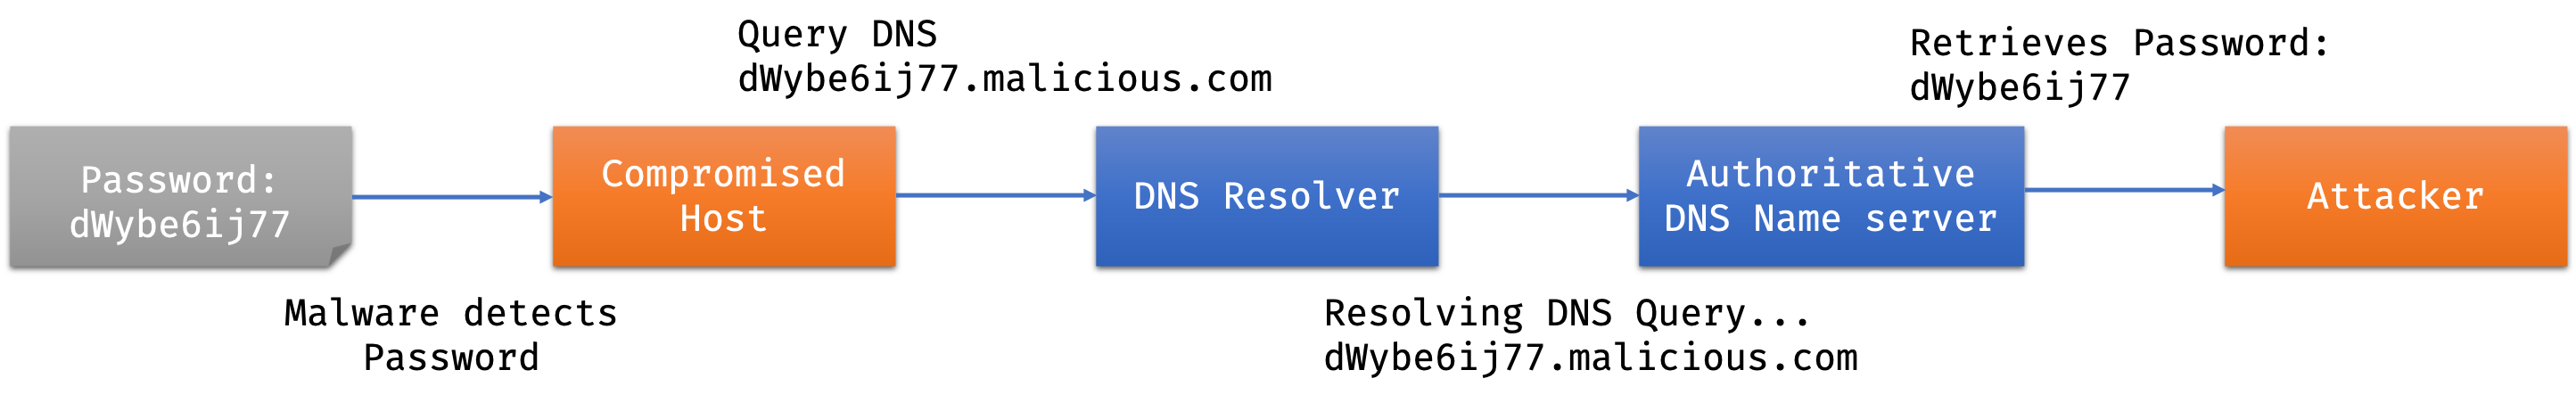
\includegraphics[width=\textwidth]{imgs/dns-data-exfil-out.png}
  \caption{Malware extracting password from host through DNS}
  \label{fig:dns-data-exfil-out}
\end{figure}

Similarly, Figure \ref{fig:dns-data-exfil-cycle} demonstrates an example where the malware queries C\&C for commands to archive remote control on the compromised host. The DNS query remains similar to the example above in Figure \ref{fig:dns-data-exfil-out}; the difference lies in the DNS reply from the \url{malicious.com} name server. The attacker can respond with a Canonical Name (CNAME) Record indicating the instruction, usually with a very short TTL, so as to avoid this instruction getting cached. This DNS query getting resolved on the compromised host will instruct the malware to act as ordered, in this particular figure, to read files and folders in \url{~/Documents}.

\begin{figure}[h!]
  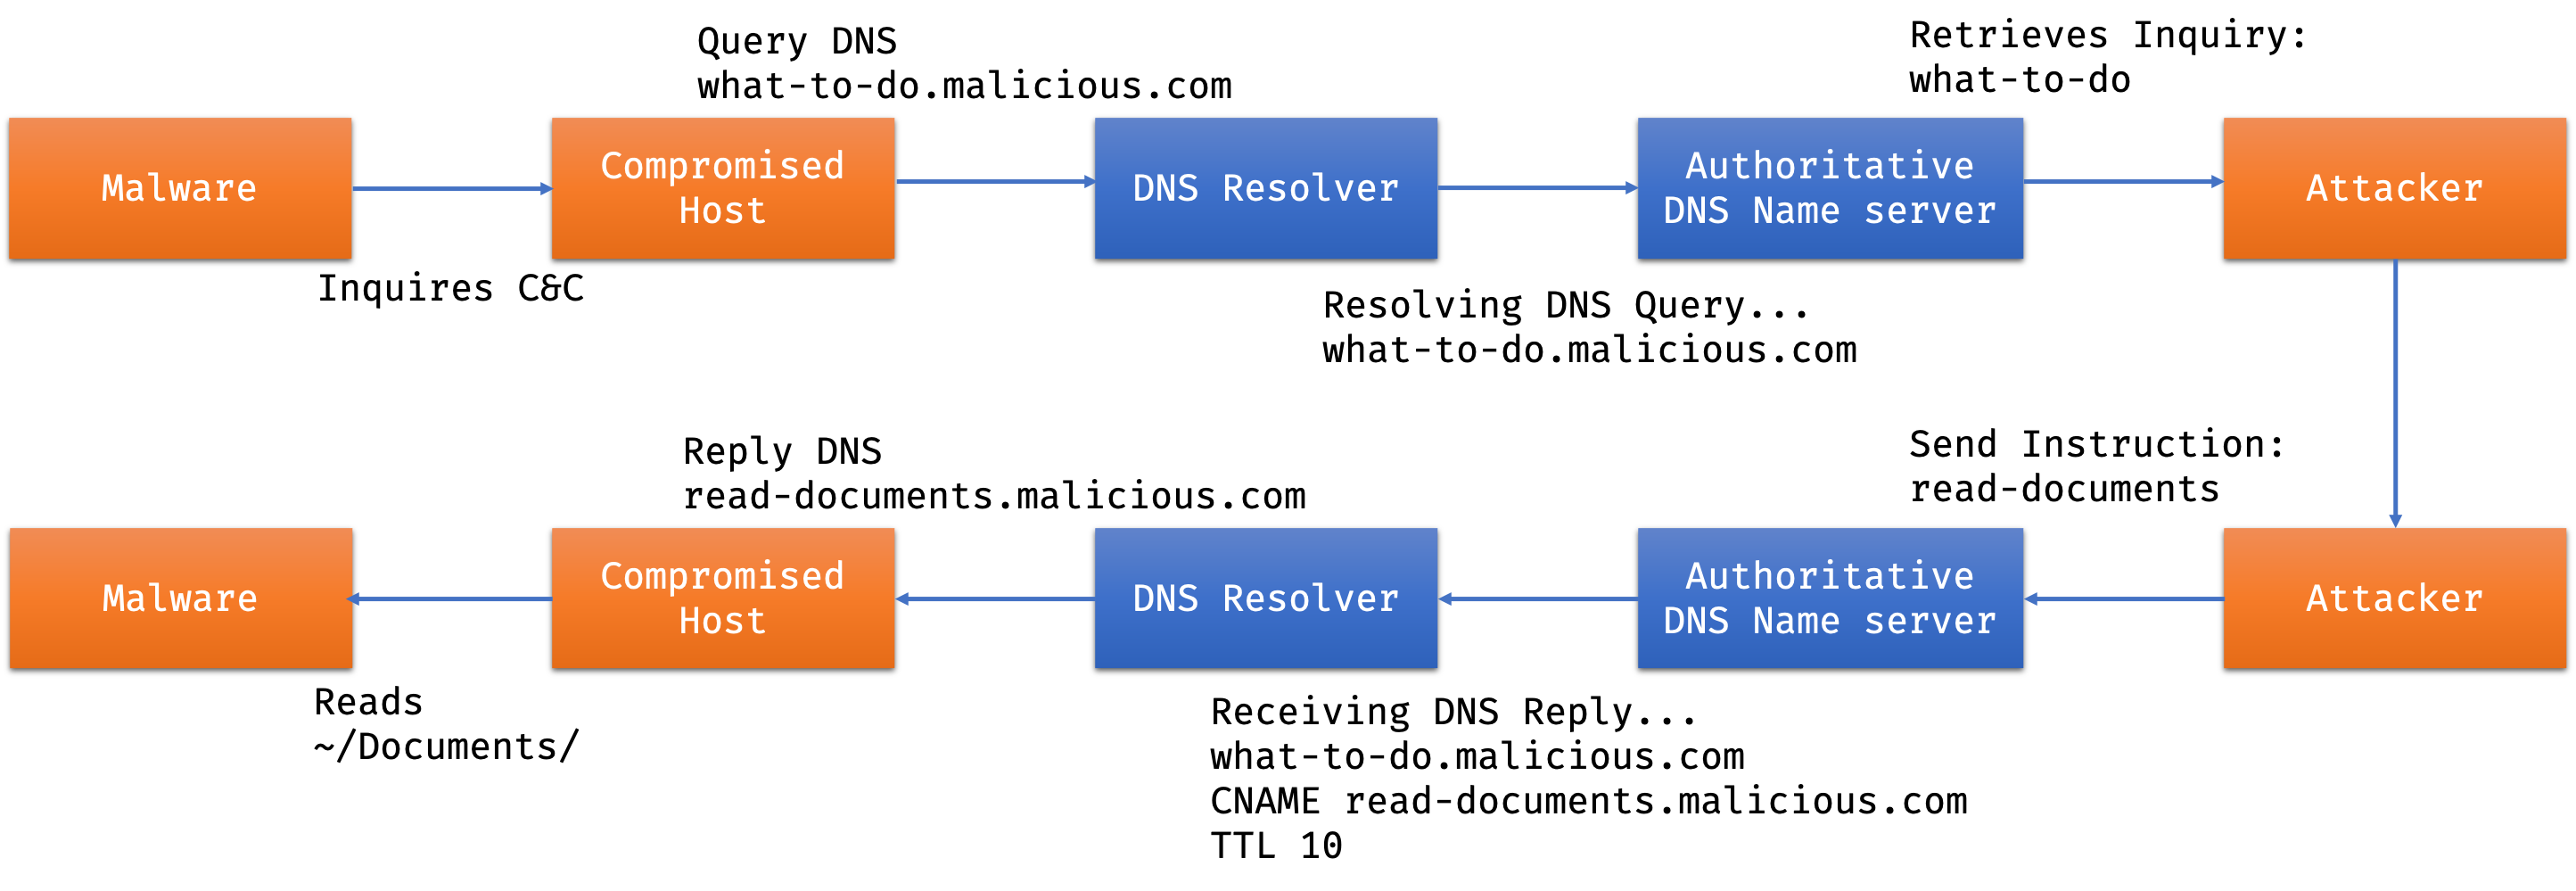
\includegraphics[width=\textwidth]{imgs/dns-data-exfil-cycle.png}
  \caption{Malware executing commands from remote C\&C}
  \label{fig:dns-data-exfil-cycle}
\end{figure}

Malware exploiting DNS for data exchanges can be divided into two major approaches: high-throughput tunnelling and low-throughput tunnelling.

As of high-throughput tunnelling, the malware would establish a bi-directional communication channel on top of the DNS via emulating a reliable and packet ordered network session between the compromised server and its C\&C. For example, the malware can enforce a Transmission Control Protocol (TCP) on top of DNS or send constant ping messages throughout communication to understand the replies' order. However, applying these methodologies would significantly increase the total amount of DNS traffic and each DNS packet's length while vastly decreasing the meantime between DNS transactions \cite{nadler-2017, nadler-201936}. As seen in Figure \ref{fig:dns-high-throughput-tunnelling}, the query intervals are less than 1 second due to the regular session keep-alive messages, the response towards the same queried domain \url{paaqfiiq.iodine.exfiltration.party} varies notably to signal a two-way communication tunnel, and some query length exceeds 200 bytes. These unusual characteristics compared to normal DNS traffic implies the existence of data exchange and exfiltration on top of DNS \cite{nadler-2017}.

\begin{figure}[h!]
  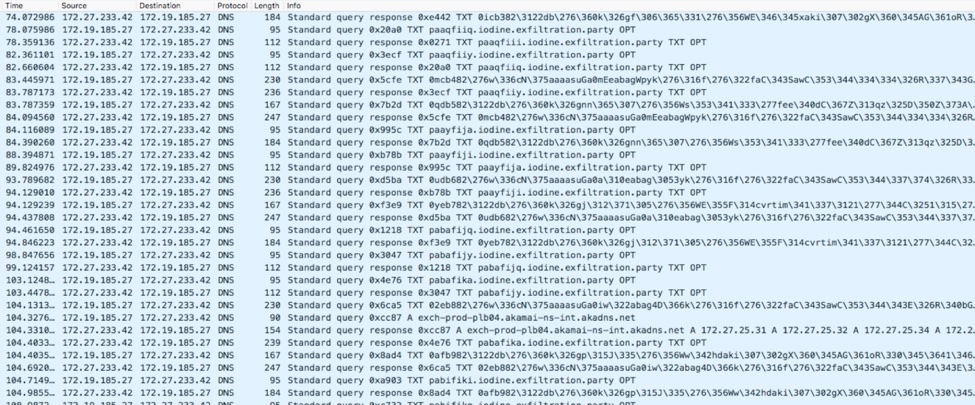
\includegraphics[width=\textwidth]{imgs/data-exfil-high-throughput-pcap.jpg}
  \caption{Sample \url{.pcap} file captured when running high-throughput DNS tunnelling}
  \label{fig:dns-high-throughput-tunnelling}
\end{figure}

Compared to high-throughput tunnelling, low-throughput tunnelling is generally harder to detect and remains overlooked within the cyber-security community \cite{nadler-2017, nadler-201936, ahmed-2020}.
To circumvent anomaly detection methods and firewalls, attackers would typically avoid using TCP tunnels or sending constant ping messages. Alternatively, the malware would wake up periodically, or triggered by specific activities, to deliver poll messages and summary of machine activities to the C\&C \cite{nadler-2018}. For example, an infected Point-of-Sale (POS) terminal would be triggered upon a swipe and send transaction and card details to the attacker's C\&C without waiting for a response.

Detecting DNS tunnelling has been widely researched over the last decade, including detecting covert tunnelling \cite{gilbert-2009, davis-2016}, and high-throughput DNS tunnelling detection \cite{wang-2016, buczak-2016, cambiaso-2016, engelstad-2017, homem-2017, kara-2014, sheridan-2015}. However, most publicly available detection solutions focus on high-throughput tunnelling due to its distinguishable network behaviour. These detection solutions rely heavily on the volume and variety of requests DNS tunnelling tools generate \cite{nadler-2017, nadler-2018}. One of the most popular solutions is DNS traffic rate control, offered by most security vendors \cite{homem-2017, nadler-2017}. More sophisticated solutions include supervised learning models on tunnelling DNS traffic, and non-tunnelling DNS traffic \cite{buczak-2016}, and anomaly detection models that would trigger upon notable change over DNS traffic as a whole \cite{davis-2016, sheridan-2015}.

\begin{table}[h]
\resizebox{\textwidth}{!}{%
\begin{tabular}{l|l|l|l}
Year & Malware       & Targets    & Malicious Domain Name   \\ \hline
2017 & DNS Messenger & Enterprise & \url{cspg.pw, algew.me}                          \\
2016 & MULTIGRAIN    & POS        & \url{dojfgj.com}                                 \\
2015 & BernhardPOS   & POS        & \url{29a.de}                                     \\
2015 & JAKU          & Botnet     & \url{LS4.com}                                    \\
2015 & Wekby         & Enterprise & \url{ns1.logitech-usa.com}                       \\
2014 & FrameworkPOS  & POS        & \url{a23-33-37-54-deploy.akamaitechnologies.com} \\
2014 & PlugX         & RDP/RAT    & \url{ns4.msftncsl.com}                           \\
2011 & FeederBot     & Botnet     & \url{images.moviedyear.net}                      \\
2011 & Morto         & RDP/RAT    & \url{ms.jifr.co.cc., ms.jifr.net.}      
\end{tabular}
}
\caption{A survery of malware from 2011-2018 exploiting DNS for low-throughput data exfiltration and exchange \cite{nadler-201936}}
\label{table:survey-malware-low-throughput-dns}
\end{table}

Although the topic of high-throughput DNS tunnelling has been studied thoroughly, little progress has been made on low-throughput DNS data exfiltration/exchange \cite{nadler-201936, steadman-2018, ahmed-2020}. A recent survey conducted by Nadler et al. \cite{nadler-201936} shown in Table \ref{table:survey-malware-low-throughput-dns} listed a number of malware exploiting DNS for low-throughput data exfiltration/exchange exposed during 2011 to 2018. These malware targets vary from enterprise networks, botnets, POS terminals to Remote Desktop Protocol (RDP) / Remote Access Trojan (RAT). Meanwhile, the set of internet domains used by these malware includes concise ones (i.e. \url{29a.de}) to maximise the data exchange rate under the 255-byte query limit, and misleading ones (i.e. \url{ns1.logitech-usa.com}) imitating well-known brands to better hide under the human inspection of DNS traffic \cite{nadler-201936}. Detecting and blocking this type of malicious DNS traffic is much more difficult given its minimal proportion across the overall DNS traffic within an extensive network. Defending against these malware would require Deep Packet Inspection (DPI) from a Layer-7 firewall to at least parse through all DNS packets. This would induce extra latency to DNS transactions and slows down performance-critical services within the network. 

Hence, in this project, we will be targetting at building a solution that detects and blocks upon request both types of DNS data exfiltration/exchange methods reliably without introducing any significant latency to the network.

\subsection{DNS Flood}
\label{section:background-dnsflood}

DNS flood attack is a type of DDoS attack, as shown in Figure \ref{fig:dns-flood}, where the junk incoming traffic floods the victim's server, making it unable to provide normal service to legitimate users for a prolonged period \cite{cloudflare-dns-flood}. Given DNS is the backbone service of translating domain names to IPv4 addresses, successfully attacking DNS name servers can make a significant proportion of the Internet unusable for most people. Furthermore, in recent years, there has been a substantial rise in IoT devices, a considerable amount of which are poorly secured \cite{mahjabin-2019}. In 2016, a botnet malware, Mirai\cite{bisson-2016}, utilises the high-bandwidth connections of IP cameras, Network Video Recorder (NVR) boxes and many other IoT devices to directly overwhelm name servers owned by DYN, a major DNS service provider. The peak flood bandwidth reached more than $12$ Gigabits per second, with more than $1$ million packets on a single DNS name server, resulting in significant take-downs of multiple popular websites, including GitHub, Netflix, Amazon, etc. \cite{bisson-2016, akamai-dns-flood}.

\begin{figure}[h!]
  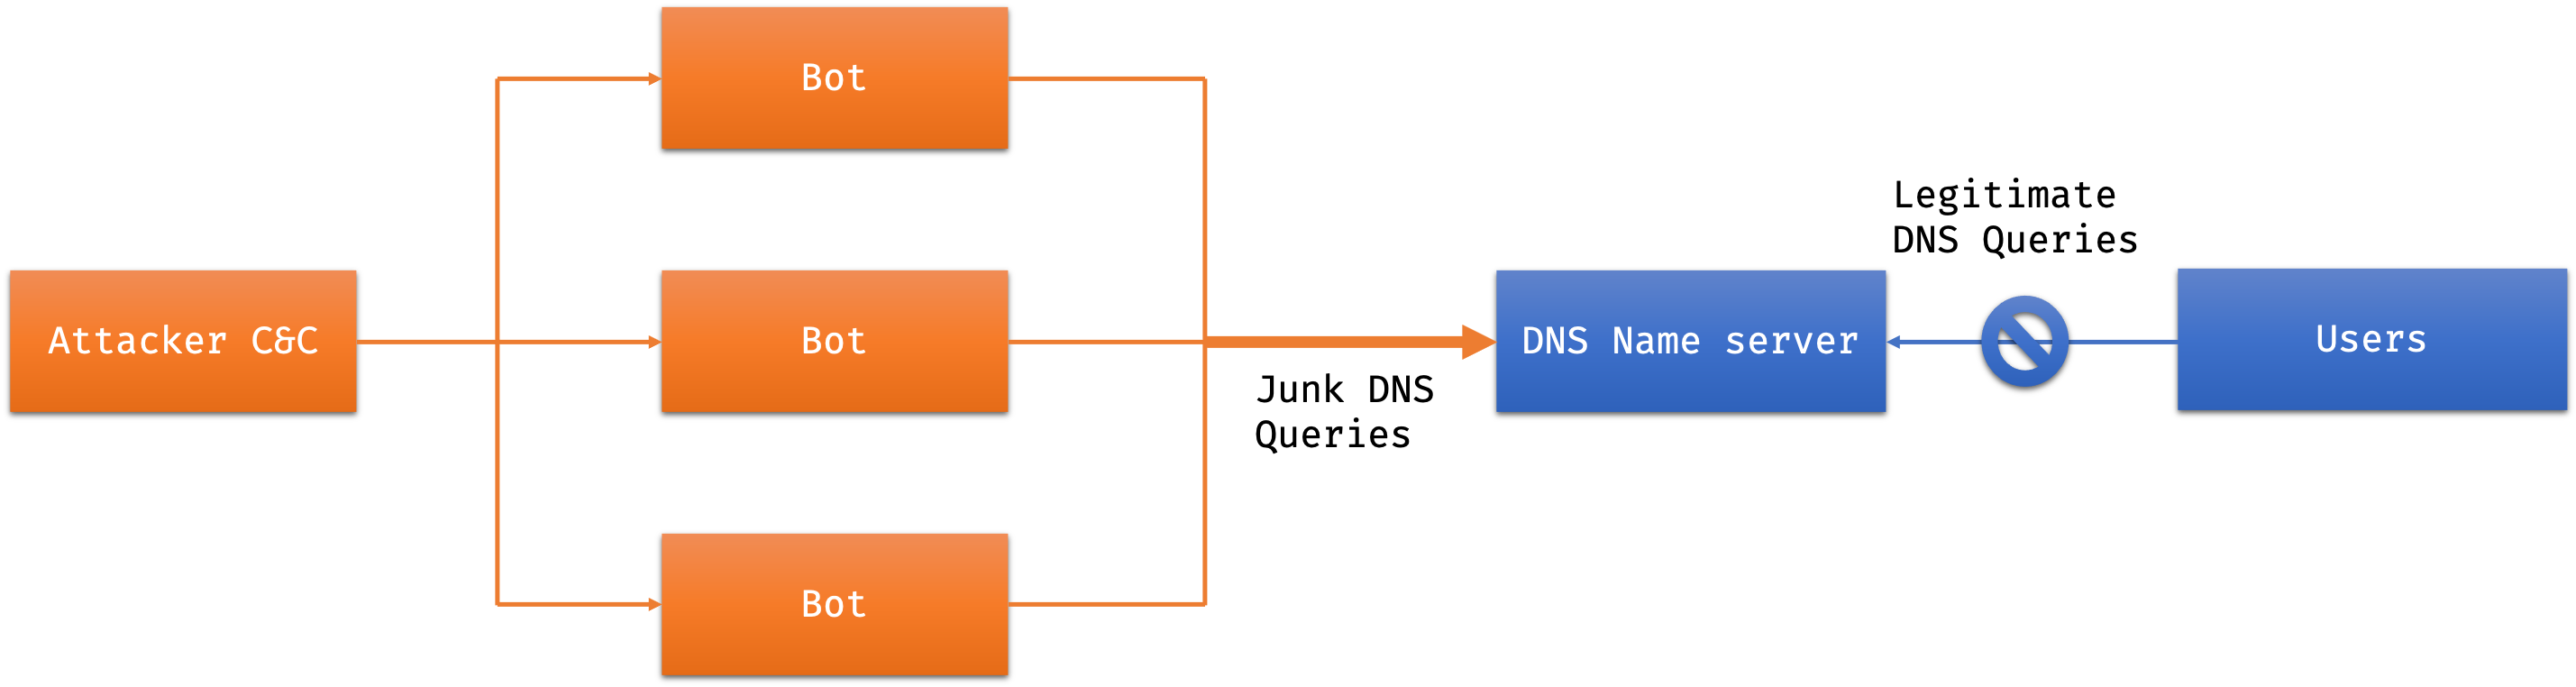
\includegraphics[width=\textwidth]{imgs/dns-flood.png}
  \caption{Botnet commencing DNS flood attack targetting a DNS name server}
  \label{fig:dns-flood}
\end{figure}

DNS flood attacks are designed to circumvent DNS resolvers' caching and continuously enable DNS queries to go to certain authoritative name servers. It is done via a technique named Pseudo-Random Subdomain (PRSD) \cite{akamai-dns-flood}. The botnet attacker targetting a domain would generate a great number of non-existent prefixed subdomain requests, causing each bots corresponding DNS resolver to continuously query the authoritative name server with a \code{NXDOMAIN} reply. In the cases where bots are conducting DNS flood are making requests to name servers directly, blocking such clients and imposing a request rate limit could be straight forward. However, it is more likely that these malicious DNS queries are coming from upstream ISP DNS resolvers or public resolves, which would not cache \code{NXDOMAIN} reply for saving resources on these resolvers \cite{akamai-dns-flood}. This complicates the DNS flood mitigation process as rate-limiting or blocking these public / ISP DNS resolvers risk throttling legitimate queries from users, which happens to share the same resolvers.

As a Cloudflare paper \cite{cloudflare-dns-flood} points out, DNS flood attack represents a change from the traditional DNS amplification based attack methods. DNS flood is an application attack (Layer 7) rather than a volumetric attack (Layer 3). There is no spoofing required for DNS flood, nor does the request comes directly from the attacking source, but upstream DNS resolvers \cite{akamai-dns-flood, cloudflare-dns-flood}. Realistically, DNS flood would not be gone until most compromised IoT devices can be secured by updating firmware or replacing easy-to-guess passwords. Therefore, besides building a large and distributed DNS name server group, we would attempt to tackle this problem via building a performant packet processing solution to absorb and block the attack traffic in real-time.

\subsection{Field Programmable Gate Arrays (FPGA)}
\label{section:background-fpga}

FPGA is a type of integrated circuit designed to be customised by a designer after its fabrication, hence "programmable on the field". As shown in Figure \ref{fig:fpga-arch}, it contains a matrix of Configurable Logic Blocks (CLBs) and higher levels of configurable interconnect, which activates and links the blocks in the manner the developer specifies \cite{xilinx-fpga}. There are two types of FPGAs, one-time programmable (OTP) ones and re-programmable ones \cite{xilinx-fpga}. Since OTP FPGAs are rare and outdated, we will mainly discuss Static Random Access Memory (SRAM) based re-programmable FPGAs.

\begin{figure}[h!]
  \centering
  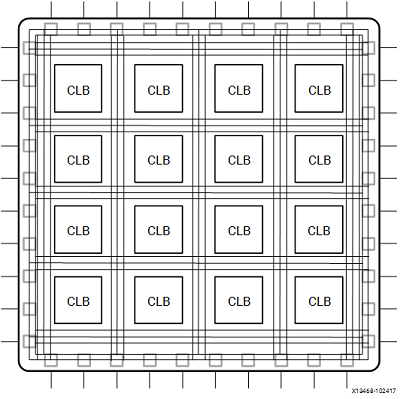
\includegraphics[width=0.3\textwidth]{docs/report/imgs/fpga-arch.png}
  \caption{FPGA Architecture \cite{xilinx-fpga}}
  \label{fig:fpga-arch}
\end{figure}

Software network middlewares including firewalls \code{netfilter}/\code{iptables} \cite{netfilter-iptables}, \code{pf} \cite{pf}, \code{ipfw} \cite{ipfw} has been widely used in industrial and enterprise networks. As the network bandwidth grows, these software-based network middlewares are heavily limited by the parallelism and processing power of a single CPU. They can no longer meet the line rate packet processing requirements for large networks with high link speeds, typically $40$ Gbps and beyond \cite{fiessler-2016}. Therefore, we've seen an increasing number of packet processing systems built upon special purpose hardware, such as network processors (NPUs) \cite {qi-2007, duo-2006}, FPGAs\cite{hager-2014, fong-2012, jiang-2009, jiang-2009-large} and even ASICs \cite{bosshart-2013}. These hardware-based solutions provide an abundant amount of parallelism and can scale up almost linearly with minimal effort. Nowadays, the highest grade 7nm ASIC packet processors can archive an overall network throughput of more than $25.6$ Tbps \cite{tomahawk-2021}, with a single packet latency lower than $400$ ps, orders of magnitude faster than any of the software-based packet processors.

There are various types of trade-offs among different implementations of network processors with regards to development time and cost, as well as flexibility and long-term adaptability. Among all three, ASIC-based Network Interface Cards (NICs) have the highest performance and power efficiency but suffers from a long development cycle, high development cost, and minimal flexibility after fabrication \cite{amara-2006, deierling-2018}. Oppositely, CPU-based or System-on-Chip (SoC) NICs are easier to program and can be deployed for highly complex use cases, as CPU provides general computability and the highest flexibility among all three \cite{deierling-2018}. FPGA-based NICs strikes a balance between ASIC and SoC by providing "field-programmable" hardware. In other words, FPGA would have performance similar to that of ASIC since they are both integrated circuit for application-specific purposes while maintaining the flexibility of being adapting and upgrading after fabrication. Due to circuit limitations, the performance, energy efficiency and achievable timing frequency of FPGAs would be inferior to that of ASICs. On the other hand, FPGAs would be much more complex to program than SoC due to hardware timing constraints and electrical uncertainties, and deployed FPGA algorithm would ultimately be limited by the number of logic units on the FPGA chip \cite{deierling-2018}.

\subsection{SipHash}

SipHash is an Add-Rotate-Xor (ARX) family of pseudo-random hash functions created in 2012 \cite{aumasson-bernstein-2012}, aimed at mitigating various "hash-flooding" DDoS attacks in late 2011 \cite{lennon-2011}. SipHash has typically used as a Message Authentication Code (MAC) calculation method to guarantee the sender's authority and message's integrity. 

Let $X$ be a message string, and $k$ be a key string, SipHash guarantees that even if an attacker have seen $X$ and $\code{SipHash}(X, k)$, an attacker who does not know $k$ would not be able to find out $k$ nor construct $\code{SipHash}(Y, k)$ for any message $Y \neq X$ which they have not seen before. Further cryptanalysis and mathematical proof of the promise above have been done by Christoph et al. \cite{dobraunig-2014} and Xin et al. \cite{xin-2019}.

SipHash has several unique characteristics that make it a suitable candidate for hardware implementation, namely simplicity, simple middle states, and minimal overhead \cite{aumasson-bernstein-2012}. The algorithm iterates a simple SipRound function utilised multiple times; hence the hardware component and circuit can be reused at different clock cycles. Siphash's middle states consists of only four 64-bit variables $v_0 ... v_4$. From a hardware implementation perspective, it minimises Flip-Flop (FF) usages, easing the design implementation on the board. Most importantly, the generated MAC is concise and of designated length (64 bits), bringing minimal and fixed consumption of hardware units.

\section{Related Work}

Although FPGA has been used to build various network appliances, only very little public research considered using FPGA against DNS exfiltration attacks. Thomas et al. \cite{thomas-2011} proposed an FPGA-based system for detecting malicious DNS network traffic, which only extracts DNS query domains and match it by hash against a list of hard-coded domain names with the memory. This approach is limited by the lack of real-time adaptability of the filter list and the inability to mitigate DNS exfiltration and flood attacks on the fly. 

With regards to using FPGA to mitigate DNS flood attacks, most related research aims at mitigating DDoS attacks as a whole instead of DNS flood attacks in particular \cite{hoque-2017, nagy-2018, tokusashi-2016, thinh-2016}. FPGAs have been used to detect DDoS attacks in real-time \cite{hoque-2017} and mitigate such attacks with very low reaction time \cite{nagy-2018}. However, most research aimed at mitigating DDoS attacks using FPGA focused primarily on DNS Amplification attacks \cite{nagy-2018, thinh-2016, tokusashi-2016}, as it was more prevalent and could be used to target individuals or smaller networks with low protection facilities in place. With reference to Section \ref{section:background-dnsflood}, the Mirai botnet's successful DNS flood attack against major DNS providers proves the inability of traditional mitigation methods against these new types of Layer 7 DDoS attacks. 

\section{Project Motivation}

This project introduces an FPGA-based solution that tackles two major rising threats exploiting the DNS protocol, DNS exfiltration attacks and DNS flood attacks. We will be improving on Thomas et al. \cite{thomas-2011}'s FPGA DNS filter by bringing real-time reconfigurability to our FPGA-based system. Innovatively, we will be further providing instantaneous	mitigation against DNS exfiltration transactions via hardware-accelerated DNS spoofing. Meanwhile, legitimate DNS transactions can proceed safely with minimal overhead.

Moreover, since most FPGA logic can be reused, namely traffic filtering and packet parsing in the aforementioned system, we further develop a separate FPGA operation mode to act as a low-latency Layer 7 firewall mitigating DNS flood attacks.

As the system will be used in high-bandwidth and latency-sensitive environments, we deem it necessary to develop an application-specific hardware solution for this task. Given the analysis in Section \ref{section:background-fpga} of ASIC and FPGA network processors, we preferred FPGA in our project implementation due to the cost and time limitations of a single-person final-year project.


\chapter{Design}

In this chapter, we will be presenting both the internal system design of the solution and the overall network design that this system will be put into practice. We will be elaborating on the design thought process and several design choices and considerations we made for the computing hardware and software control system. Also, we will be discussing some example topologies to illustrate how the solution will work to secure the network.

\section{System Design}

\subsection{Hardware Design}
\label{section:design-system-design-hardware}

\begin{figure}[h!]
  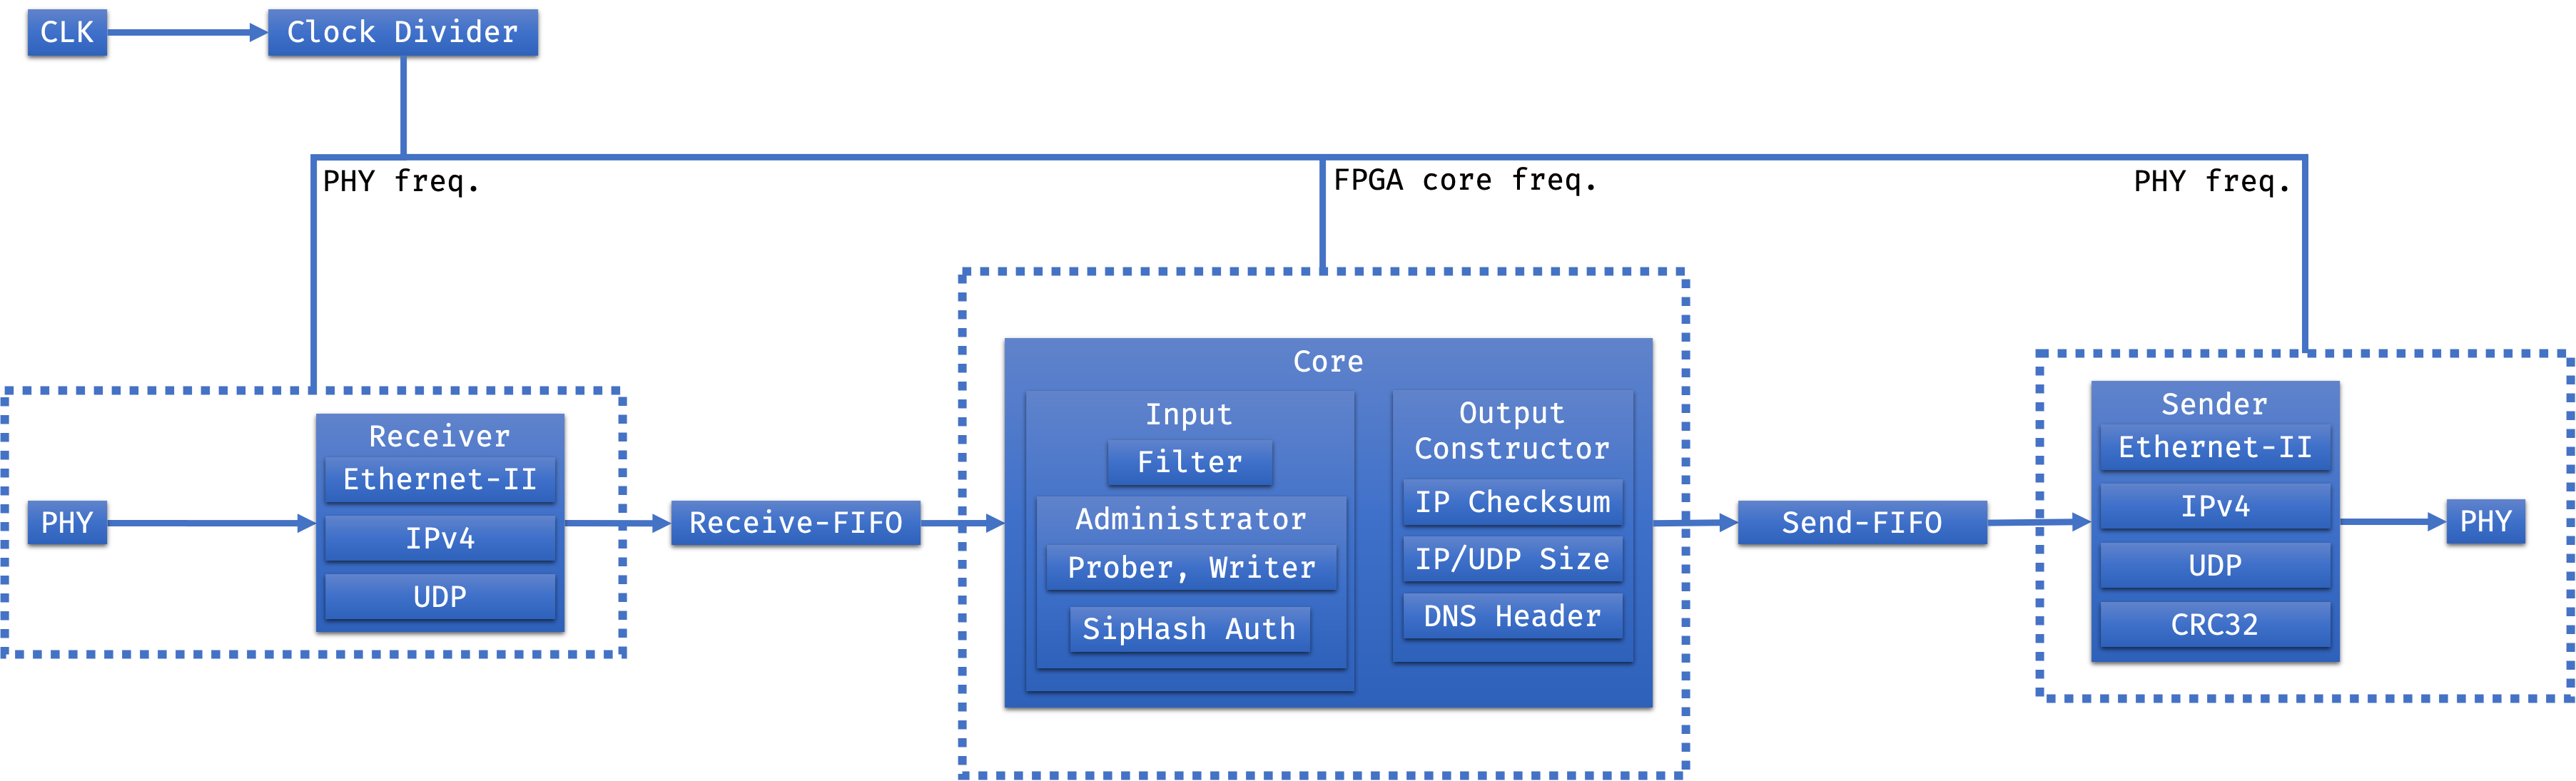
\includegraphics[width=\textwidth]{imgs/hardware-design.png}
  \caption{Hardware Architectural Design}
  \label{fig:hardware-design}
\end{figure}

Since we are designing a network processing circuit, it is crucial that we are aware of the hardware interface we are interacting with. With Ethernet-II PHY ASIC available on most development boards with RJ45 connectors, we assumed that our design would retrieve incoming bits from a certain type of Media-Independent Interface (MII) family\footnote{See Section \ref{section:implementation-hardware-implementation} for introduction to MII family and implementation details} \cite{}. Similarly, we will be outputting bits to an MII-type interface as well at the end of processing. Hence, we can derive an initial architecture of a core processing component receiving from an input circuit and sending to an output circuit, as shown in Figure \ref{fig:hardware-design}.

Retrospectively speaking, clock domains was not thought through carefully at the design stages and later became a pitfall that cost significant amount of effort on regression and fixing. It's worth considering each component's clock domain, and several clock domain crossing methods when designing the system. Generally, PHY ASIC chips operates at a lower clock frequency than the FPGA core, resulting in different clock domains within the system. The initial clock signal from the FPGA's clock path is designed to go through a clock divider that generates suitable clock signals for each of the components in various domains. Inevitably throughout the design, there would be signals crossing clock domains (i.e. from receiver to core module). If left unsynchronised, the destination domain would experience various meta-stability issues\footnote{See Section \ref{section:implementation-hardware-debugging} for more information on Clock Domain Crossing (CDC) and signal metastability in hardware}. Thus, we introduce two asynchronous First-In-First-Out (FIFO) buffers that connections receiver to core, core to sender respectively, as shown between the clock regions in Figure \ref{fig:hardware-design}.

Within the Receiver and Sender component shown on the left and right side of Figure \ref{fig:hardware-design}, we aim to design a sequential circuit that utilises a Finite State Machine (FSM)  that mainly comprised of three parsing / packing stages, Ethernet-II, IPv4 and UDP. The sender ideally shall have an extra Ethernet Cyclic Redundancy Check 32-bit (CRC32) \cite{ieee802.3ethernet-2018} generation module that appends a 32-bit checksum to the packet. As of the core processing module, we would split it into two sub-component, one handling DNS parsing, Layer 7 filtering, FPGA administration and security checks, while the other one working on constructing proper DNS / payload response and calculating sizes and checksums for higher layer protocols (IPv4, UDP and DNS), as demonstrated in the Core section of Figure \ref{fig:hardware-design}.

\begin{figure}[h!]
  \makebox[\textwidth][c]{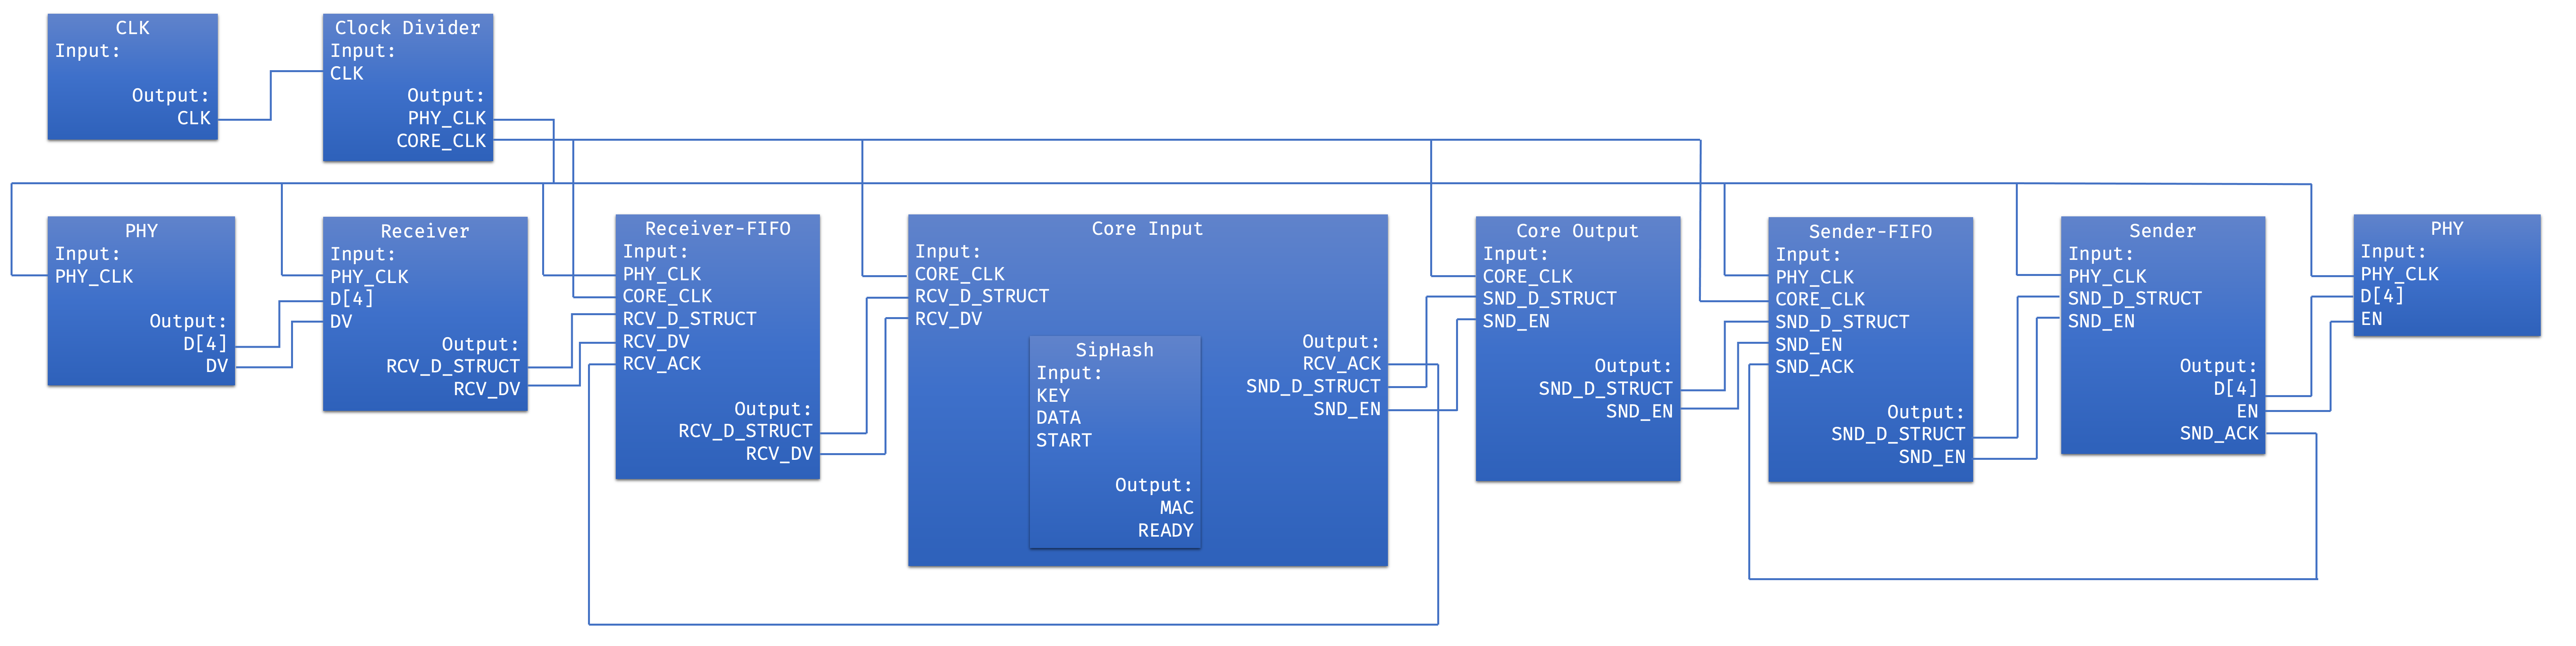
\includegraphics[width=1.1\textwidth]{imgs/hardware-signal.png}}
  \caption{Hardware Signal Design}
  \label{fig:hardware-signal-design}
\end{figure}

After designing the top-level components and their main functionalities, we will be sketching the signal schematic of the design so as to determine each component's incoming and outgoing ports, as laid out in Figure \ref{fig:hardware-signal-design} The common input for almost all synchronous sequential logic is the clock pin (\code{CLK}). As suggested previously in the section, components within different clock domains shall receive \code{CLK} with their corresponding frequencies. The only exception here being the cross-domain asynchronous FIFOs which shall be activated by both \code{CLK} signals, one for writing to the FIFO queue and the other one for reading.

To avoid actively reading and writing data when not required, we utilised various Data Valid (DV), Enable (EN) and ACKnowledgement (ACK) signals in our components, as seen in Figure \ref{fig:hardware-signal-design}. Each sequential component in hardware is designed to constantly check against a set of signals when in idle state. The set of signals shall be specified by the hardware designer as the sensitivity list of a \proglang{VHDL}'s process, or a \proglang{Verilog}'s always-block. When the activation signal reaches Voltage Common Collector (VCC) level upon a rising clock edge, the sequential component shall transit into a working state and start reading and processing the bits from other incoming signals. For example, in the core input (\code{corein}) module (Figure \ref{fig:hardware-signal-design}), we utilise two sensitive signals, \code{CLK} and \code{RCV\_DV} to ensure the data processing starts when both are at VCC level. The receiving data will then be read and further processed at later rising clocked edges.

Besides clocking and activation signals, we also need to design data transfer ports across signals. We define a custom data struct (\code{D\_STRUCT}) to maintain all signals we need for processing and discards the rest unneeded packet information. The \code{D\_STRUCT} is an internal representation of the packet with relevant metadata and parsed DNS payload. This design allows us to keep a fixed length representation of variable length packets within the hardware system\footnote{See Section \ref{section:implementation-hardware-debugging} for issues with variable length descriptors in hardware}. Moreover, we made very effort to keep the \code{D\_STRUCT} nimble so as to avoid using unnecessary FIFOs delaying data transfers or wasting FPGA resources. Given the trade-off being the lack of support for payload longer than a pre-determined limit (128 bytes in our implementation\footnote{See Section \ref{section:implementation-hardware-implementation} for our detailed implementation of packet segmentation and the 128-byte limit}), we think it's worthwhile to proceed with this appoarch as we focus primarily on processing typically shorter DNS packets with minimal latency.

\subsection{Software Design}

\begin{figure}[h!]
  \makebox[\textwidth][c]{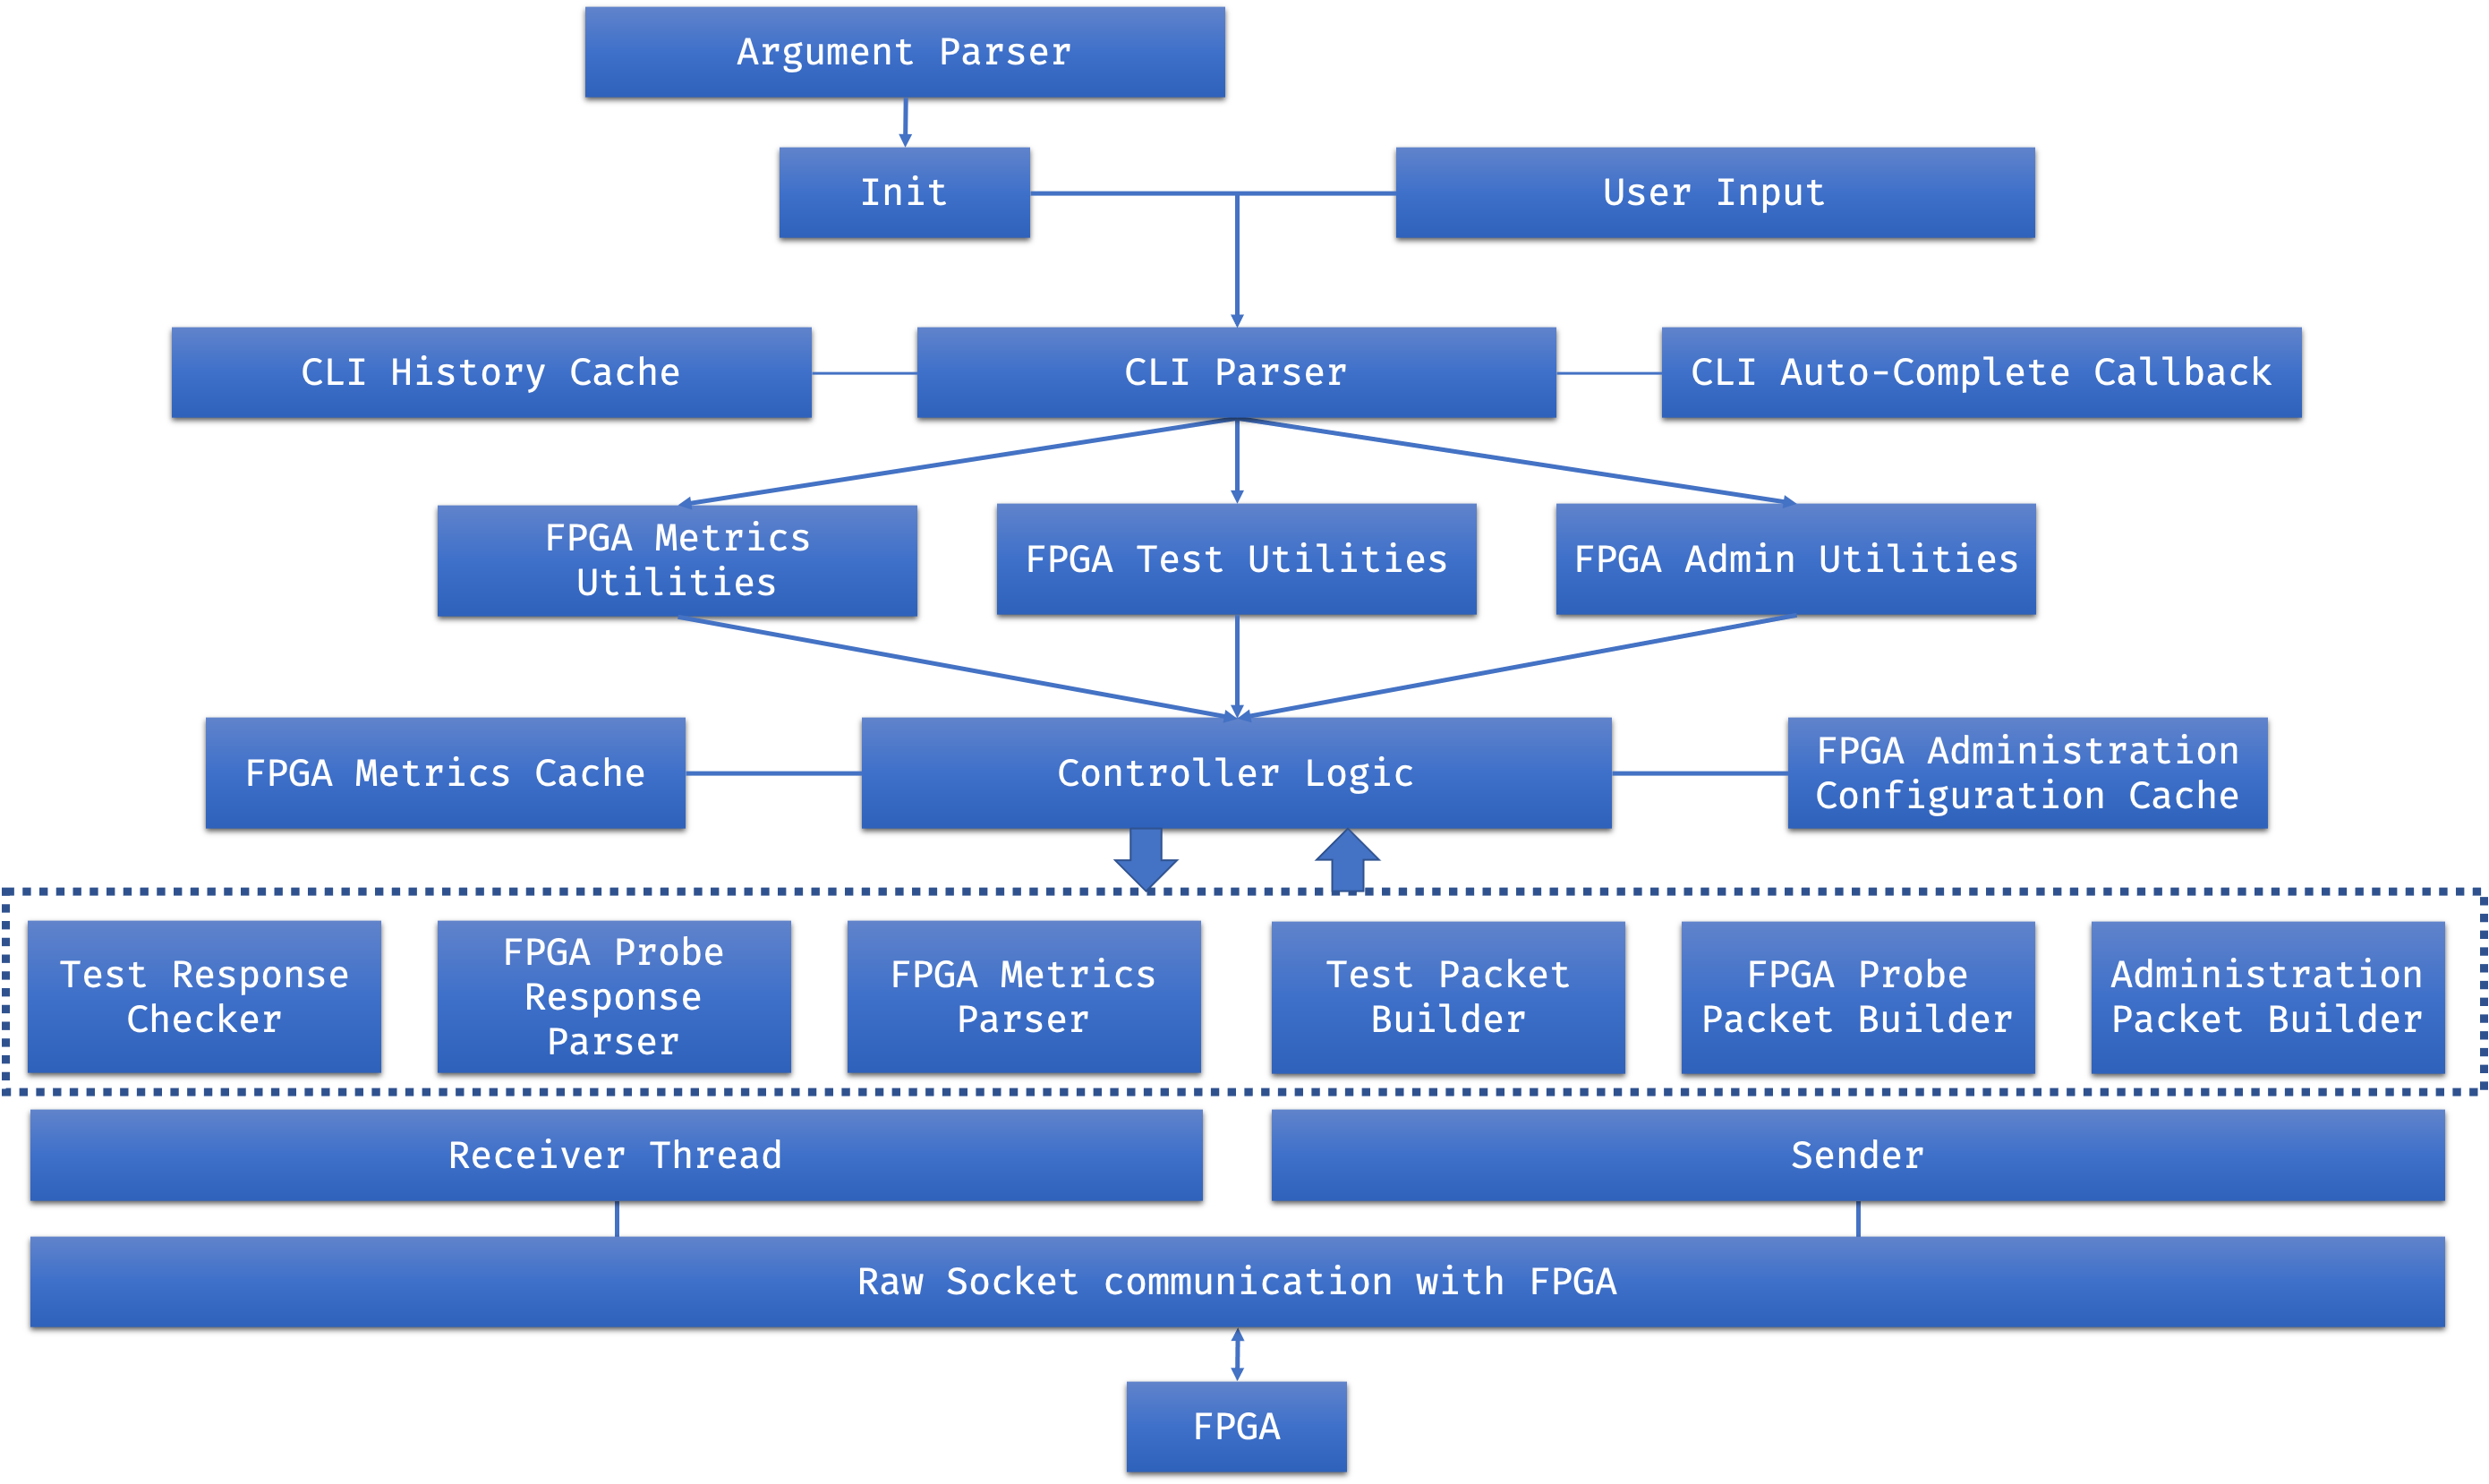
\includegraphics[width=1.1\textwidth]{imgs/software-design.png}}
  \caption{Software Design}
  \label{fig:software-design}
\end{figure}

As part of our goal to develop a resilient system, we also designed an administrative software to control, monitor and reconfigure the FPGA in real-time. As with most network configuration software, we provide a Command Line Interface (CLI) front end to administrators. The top layers of Figure \ref{fig:software-design} the software front-end is comprised of a argument parser that understands launch options, a CLI parser that splits commands into function calls and their corresponding argument string, and several supporting features, namely CLI history and CLI auto-complete functionalities.

The software is designed to provide three main command families, \code{stats}, \code{test} and \code{admin}, corresponding to the three utilities in the middle layer of Figure \ref{fig:software-design}. 
\begin{itemize}
    \item \code{stats} commands provides user with the ability to understand the accumulated statistics and metrics on the FPGA filter, including packets received, DNS replies sent and etc.
    \item \code{test} commands enables user to test the hardware implementation of the FPGA system with integration tests and stress tests. This is to make sure the system on FPGA is functioning as expected and within the performance threshold.
    \item \code{admin} commands allows user to read and write DNS filter and operation mode configurations on the FPGA. It also provides convenience features for admins to save and load FPGA admin configurations as files on the controlling system.
\end{itemize}

Since certain commands such as \code{admin show curr} (which shows the currently editing admin configuration) do not need direct information exchange with the FPGA, we utilises a central controller logic to determine back-end operations and avoid unnecessary probes of the FPGA. Therefore, as shown in the bottom layers of Figure \ref{fig:software-design}, we provide various packaged functions that interfaces with the FPGA for the controller to interact with. These functions are mainly divided into senders and receivers, which relies two different raw sockets.

The receiver socket operates like a daemon thread that is listening to all network traffic on the FPGA interface. Noteworthy replies and metrics from the FPGA will be highlighted and saved to cache automatically upon capture. Then, relevant parsers or checkers will be called to verify or understand FPGA messages accordingly. 

The sender socket, on the other side of the spectrum, is only called when necessary. When an command is issued by the controller logic, the corresponding packet builder would build an administrative, test or probe packet that will be sent to the FPGA. A response might later be received and then coordinated by the receiver as discussed above.

With the aim to provide a future proof system, we also designed Application Programming Interfaces (APIs) for more complex algorithms such as entropy-based anomaly detectors to fetch and analyse the metrics captured by the FPGA. After the analysis, the algorithms can proactively re-configure the FPGA with several simple function calls. The APIs are designed as an extension, enabling developers to engineer complex algorithms making smarter decisions and push operational changes to FPGA instantaneously.

\section{System Usage Sample Topology}

\subsection{DNS Data Exfiltration}

The main innovative application of the FPGA-based system is to detect and mitigate DNS exfiltration attacks in real-time. Typically, the system would be deployed in a secured enterprise network with confidential information on its hosts (i.e. a cloud-based POS network, a military network with restricted Internet access). Assuming the network is originally setup with a firewall comprised of ASIC-based Layer 3 firewall and software-based Layer 7 firewall, bridging the connection between Wide Area Network (WAN) and the internal network switches. The FPGA shall connect to the network in a man-on-the-side manner with its operation mode set to "Man-on-the-Side DNS spoofing".  In this particular configuration, as an example, the FPGA checkers are set to:

\begin{itemize}
    \item MAC checkers: Disabled
    \item IP checkers: Check against a known list of internal DNS server IPs
    \item UDP Port checkers: Check for port 53
    \item DNS checkers: Check for \url{enterprise.local} and \url{essential.service}
\end{itemize}

If a DNS transaction satisfies all checker requirements, the packet would then be deemed legitimate and passed on to its intended recipients. If not, the FPGA would send out a Spoofed \code{NXDOMAIN} reply (or any administrator configured DNS \code{RCODE} reply) to the host.

We can further configure the ASIC-based Layer 3 firewall, or use a Network Test Access Point (TAP) device with the FPGA filter to archive the following:

\begin{itemize}
    \item When sending a DNS packet to WAN:
        \SubItem    {If it is not sent from the FPGA, redirect it to the FPGA}
        \SubItem    {If it is sent from the FPGA, send to WAN}
    \item When receiving a DNS packet from WAN
        \SubItem    {Redirect it to the FPGA}
\end{itemize}


\begin{figure}[H]
  \makebox[\textwidth][c]{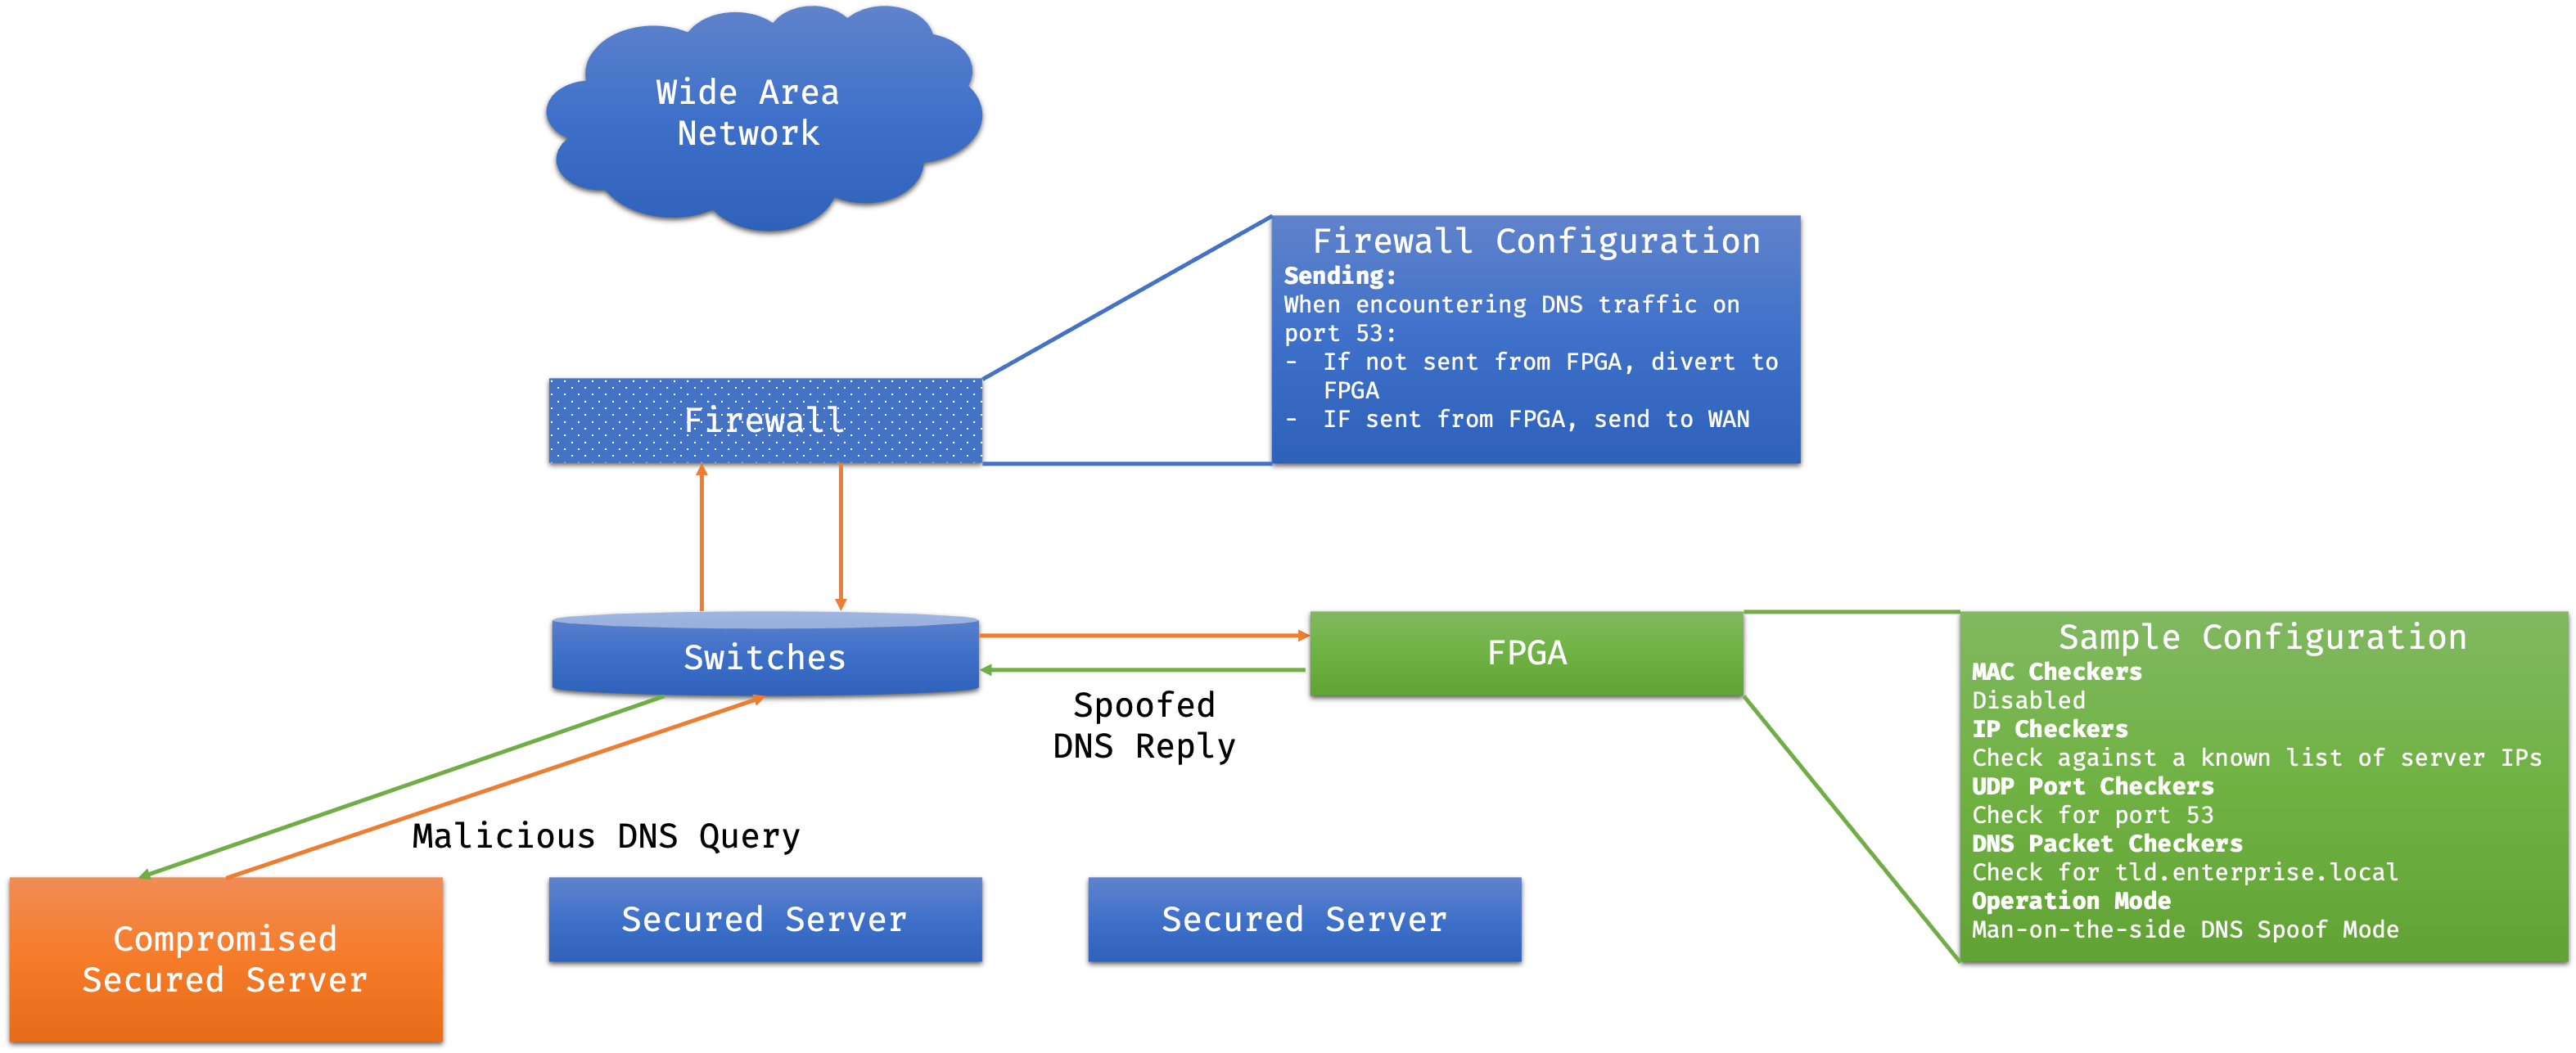
\includegraphics[width=1.1\textwidth]{imgs/man-on-the-side-malicious-dns-query.png}}
  \caption{Man-on-the-Side FPGA sample topology - Sending malicious DNS exfiltration / tunnelling query}
  \label{fig:man-on-the-side-FPGA-send-malicious}
\end{figure}

Generally, the initiative of data exfiltration usually starts from a compromised host within the network. In the event where the host sends a malicious DNS query exfiltrating data / establishing a tunnel in Figure \ref{fig:man-on-the-side-FPGA-send-malicious}, the firewall would first redirect the query to FPGA. The FPGA would spot this DNS query suspicious and send a spoofed DNS reply back to the compromised host stopping the data exfiltration. 

\begin{figure}[H]
  \makebox[\textwidth][c]{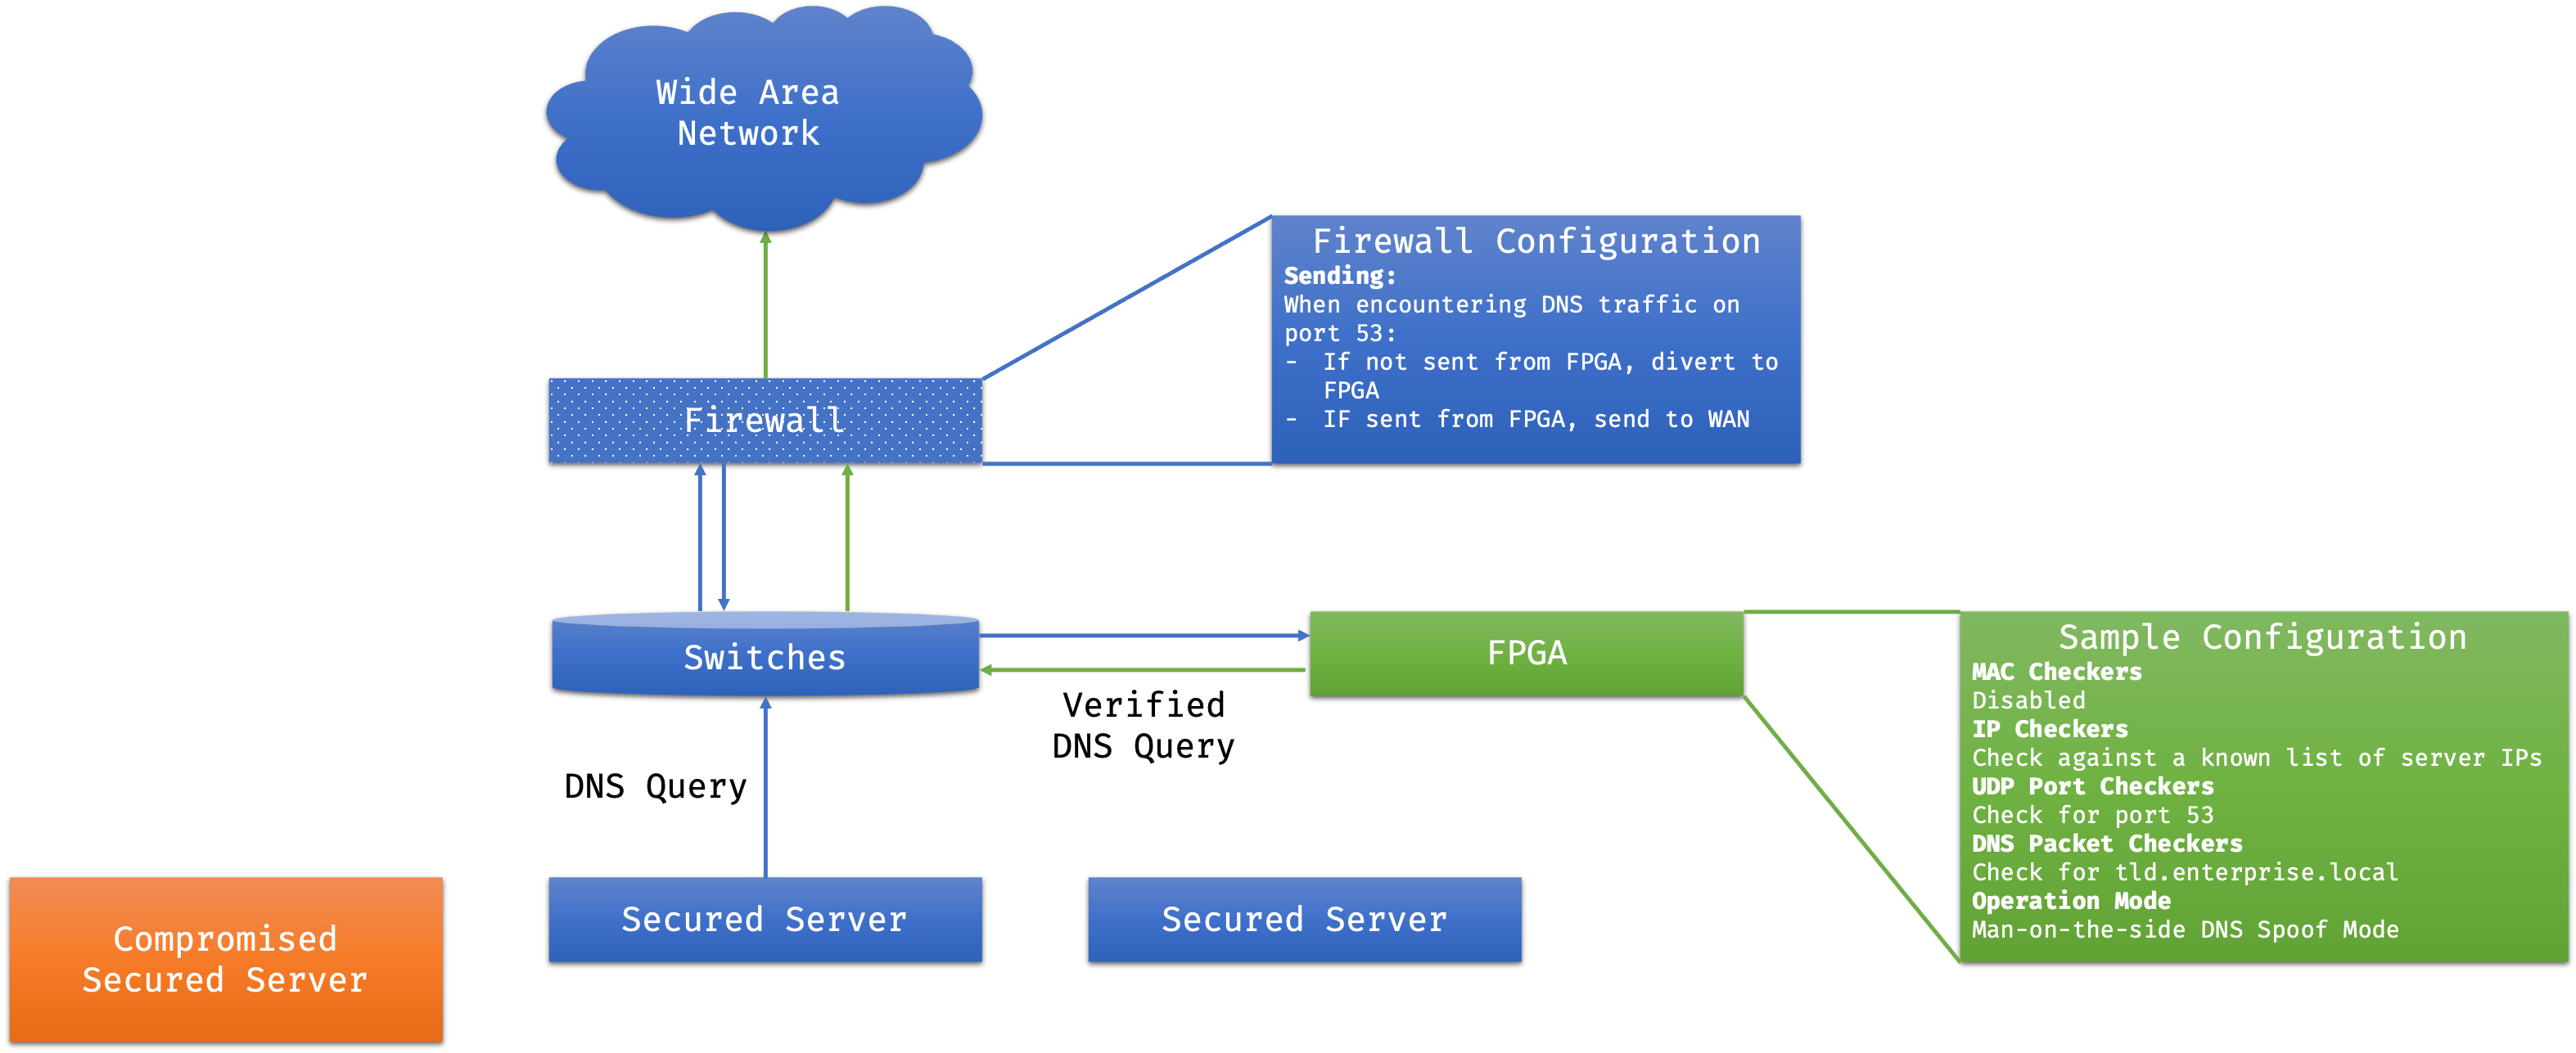
\includegraphics[width=1.1\textwidth]{imgs/man-on-the-side-valid-dns-query.png}}
  \caption{Man-on-the-Side FPGA sample topology - Sending legitimate DNS query}
  \label{fig:man-on-the-side-FPGA-send-legit}
\end{figure}

Legitimate DNS queries would not be affected within the network, as shown in Figure \ref{fig:man-on-the-side-FPGA-send-legit}. The packet will first be redirected to the FPGA for security checks. Once the FPGA deems the packet legitimate, it will forward the packet to the firewall, which will dispatch the packet to the upstream network. 

\begin{figure}[H]
  \makebox[\textwidth][c]{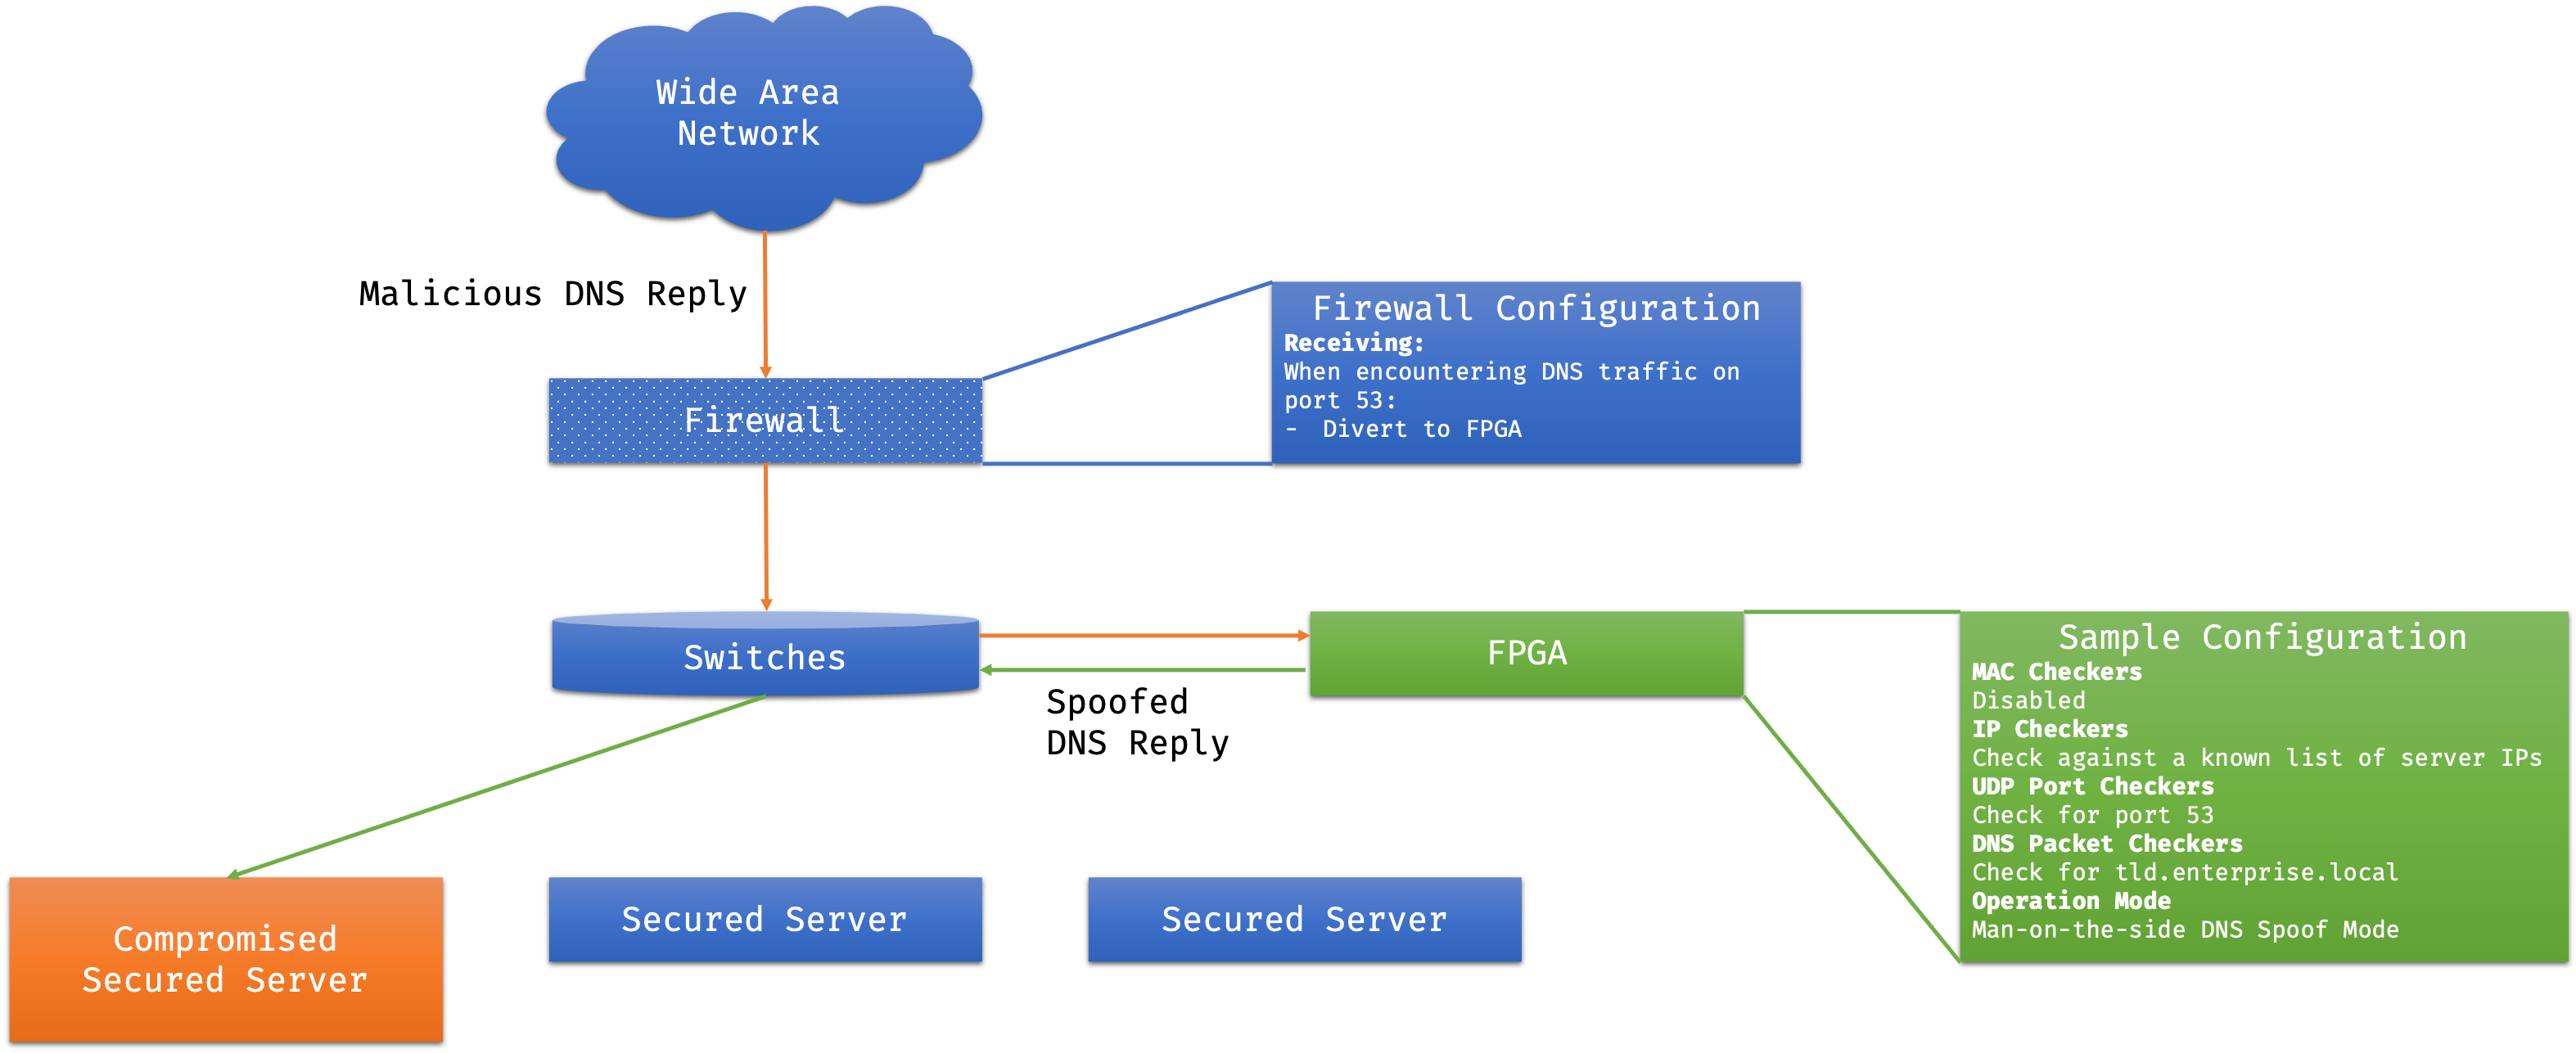
\includegraphics[width=1.1\textwidth]{imgs/man-on-the-side-malicious-dns-reply.png}}
  \caption{Man-on-the-Side FPGA sample topology - Receiving malicious DNS exfiltration / tunnelling reply}
  \label{fig:man-on-the-side-FPGA-recv-malicious}
\end{figure}

In the extremely rare case where a malicious DNS exfiltration/tunnelling query did get sent to the attacker's C\&C due unknown issues, the reply can still be blocked by the FPGA if configured properly. In the case where the networks receives a DNS remote control reply, the firewall would divert the packet to FPGA for examination. The checker in the FPGA would fail and this would also trigger a spoofed DNS reply sent to the compromised host, as shown in Figure \ref{fig:man-on-the-side-FPGA-recv-malicious}.

\begin{figure}[H]
  \makebox[\textwidth][c]{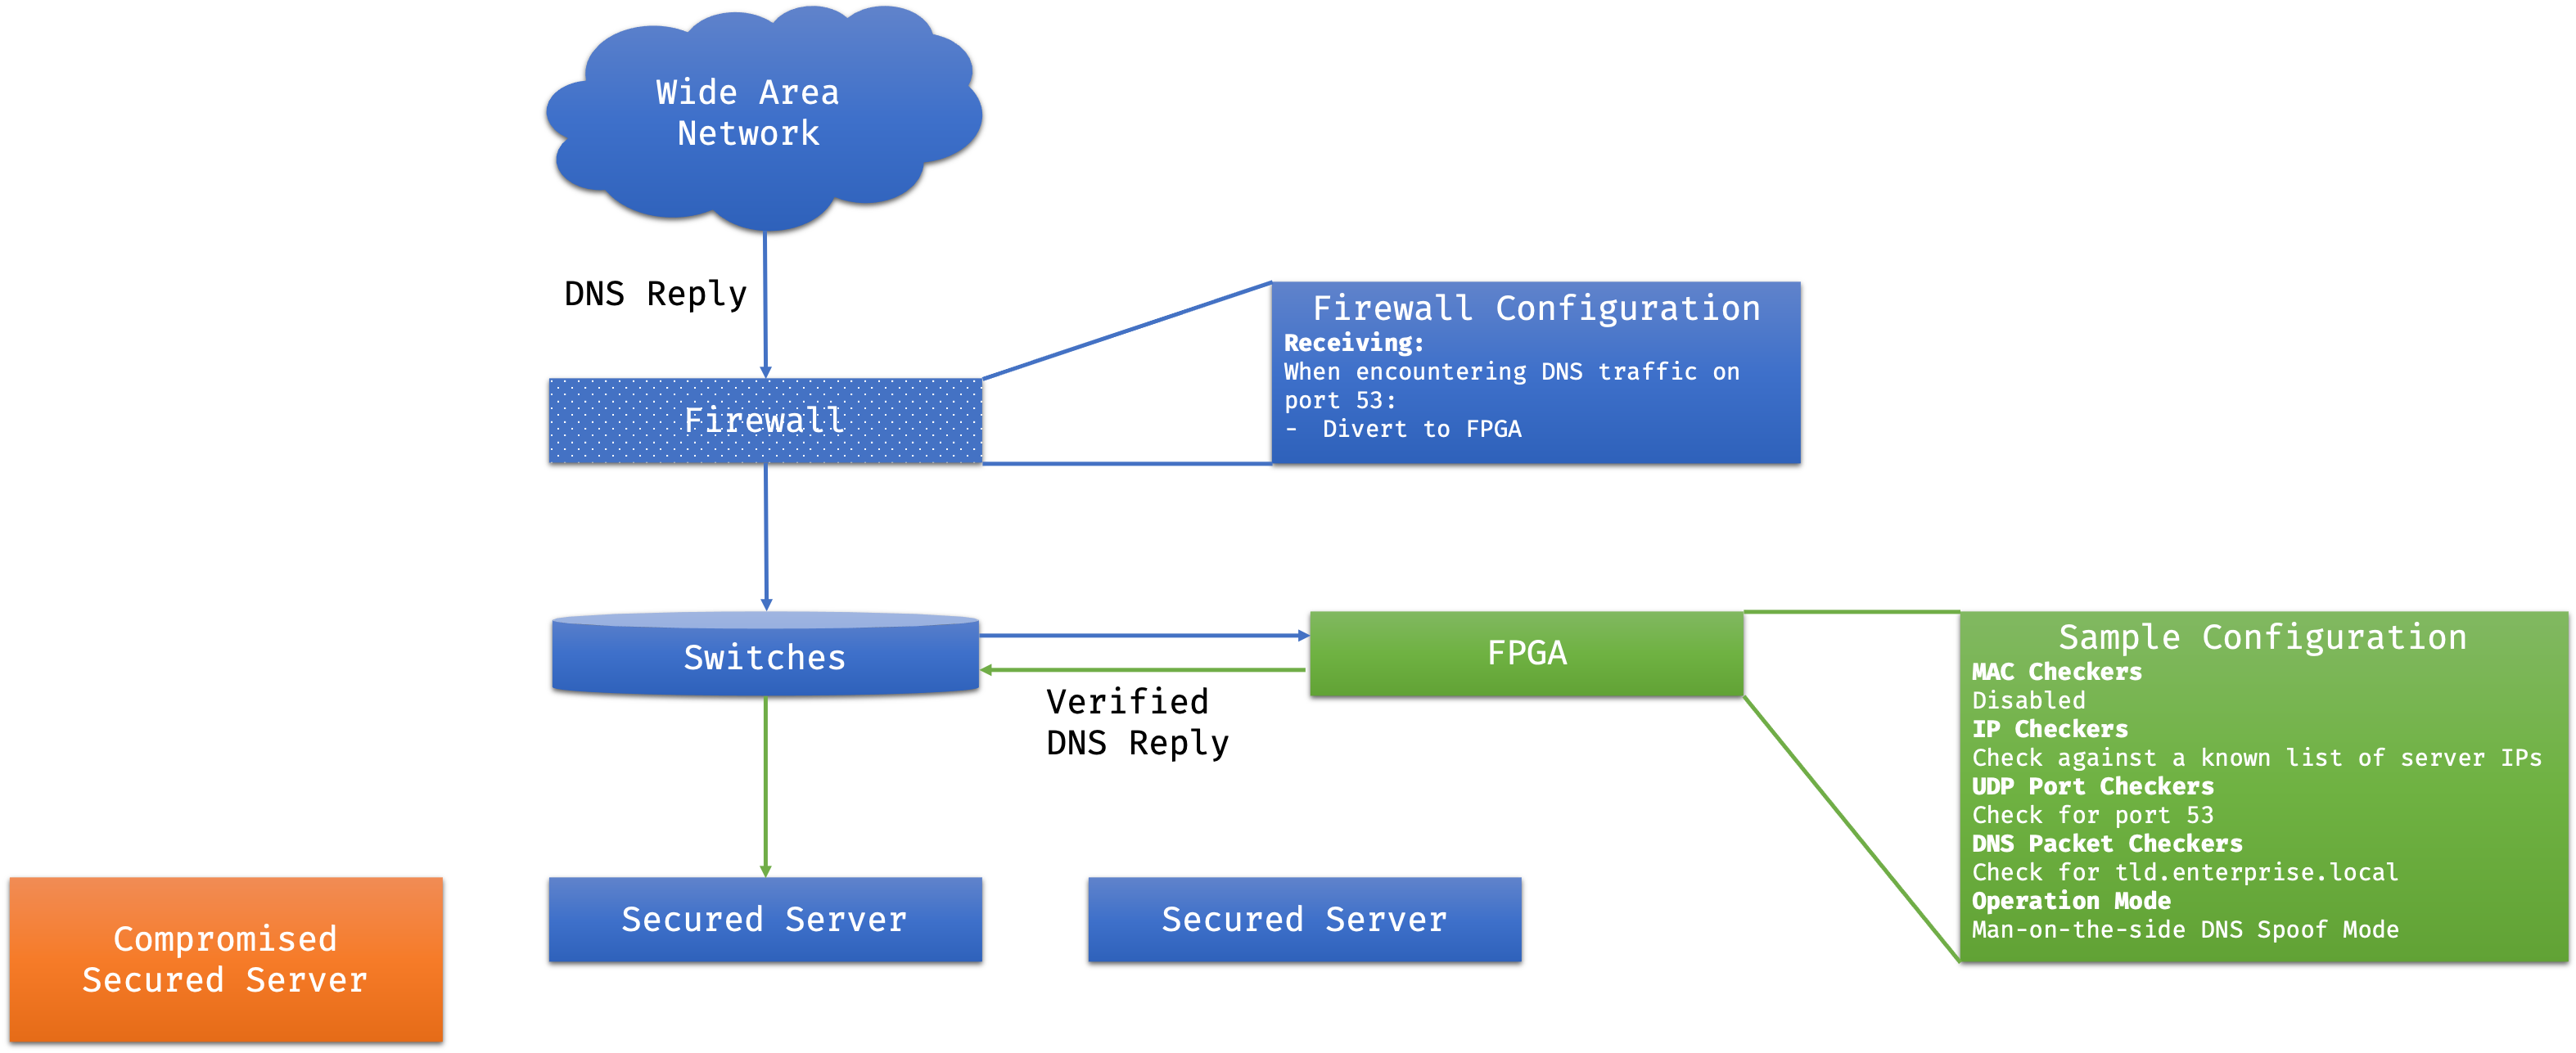
\includegraphics[width=1.1\textwidth]{imgs/man-on-the-side-valid-dns-reply.png}}
  \caption{Man-on-the-Side FPGA sample topology - Receiving legitimate DNS reply}
\end{figure}

As expected, legitimate DNS responses would remain unaffected throughout the process except for a minimal overhead added by the FPGA scrutinising the packet. The reply will be received by the firewall, forwarded to the FPGA. The FPGA will inspect the packet rapidly and deliver the verified response to the intended host untouched.

\subsection{DNS Flood}

This FPGA-based system can also be used to counter DNS flood attack on DNS name servers. As specified in Figure \ref{fig:dns-flood-man-in-the-middle}, we deploy the system in a man-in-the-middle manner in front of the DNS name servers. The FPGA operation mode is set to "Man-in-the-middle Filter", which would forward the exact payload upon passing the filter. With regards to the filters, we can configure them as:

\begin{itemize}
    \item MAC filters: Allow trusted Ethernet MACs from upstream ISP providers
    \item IP filters: Block a list of known IP address sending malicious IP addresses
    \item UDP Port filters: Allow only DNS port 53
    \item DNS filters: Allow only white-listed domain names and blocks all unknown domain names
\end{itemize}

Notably, we are placing the FPGA system as a hardware-based simple Layer 7 firewall in front of the system's software-based firewall. Utilising the unparalleled packet processing speed of FPGAs, the majority of flood traffic can be examined, logged and discarded by the FPGA with minimal latency before reaching the software firewall. Moreover, FPGAs can be scaled up linearly without extra overhead to accept and filter more flood traffic by simply connecting more FPGAs in parallel between the WAN and the software firewall. Therefore, the software firewall would enjoy much lower network load when under attack, as a large percentage of the junk traffic has already been blocked by the FPGAs. Thus, more complex checkups can be performed by the software firewall with its spare CPU time. With this setup, we can make sure the DNS name servers are well-protected with minimal performance and latency impact on the overall system.

\begin{figure}[H]
  \makebox[\textwidth][c]{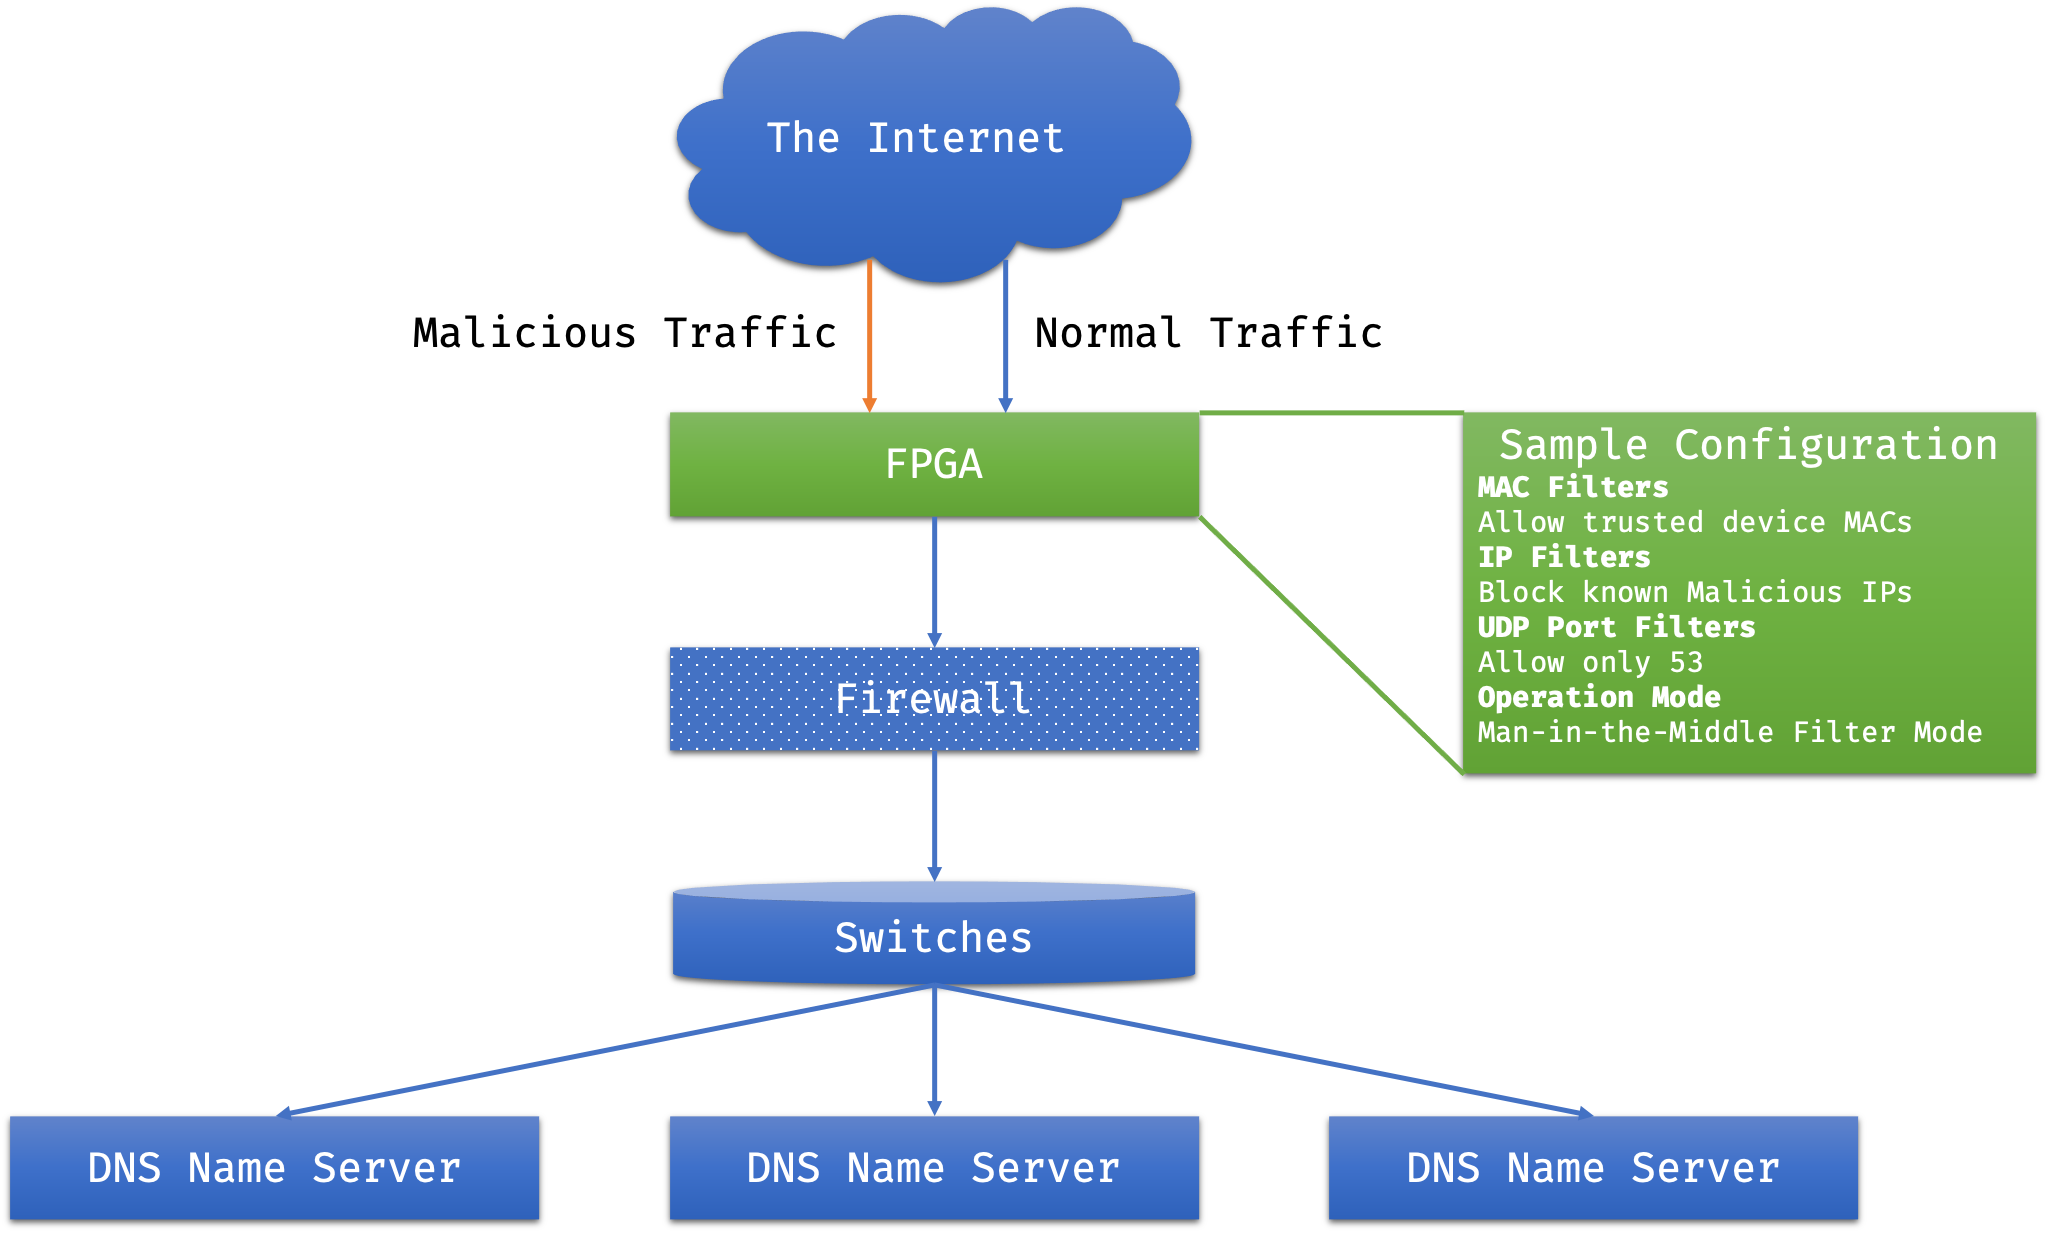
\includegraphics[width=0.8\textwidth]{imgs/man-in-the-middle-topology.png}}
  \caption{Man-in-the-Middle DNS Name Server FPGA sample topology - FPGA in the middle}
  \label{fig:dns-flood-man-in-the-middle}
\end{figure}

When it comes to certain  networks that serves not only DNS queries, the aforementioned topology in Figure \ref{fig:dns-flood-man-in-the-middle} might not be the best solution since all traffic except DNS are discarded by the FPGA. Instead, we can resort to the sample topology shown in Figure \ref{fig:dns-flood-man-in-the-middle-asic}. In this approach, we put FPGA on the side of the network only monitoring DNS transactions. Technically, this approach shall be no different as FPGA is still in the middle of all DNS traffic. The incoming traffic from WAN would ideally pass through an ASIC-based Layer 3 firewall which diverts all DNS traffic to the FPGA, and keeps other traffic on the normal route towards a Layer 7 firewall or directly towards a switch (in a less secure environment). Similar to the previous configuration, the FPGA would detect, log and drop packets not meeting the filter requirements. Legitimate payload is expected to pass the filter and get forwarded directly to the switch.

\begin{figure}[H]
  \makebox[\textwidth][c]{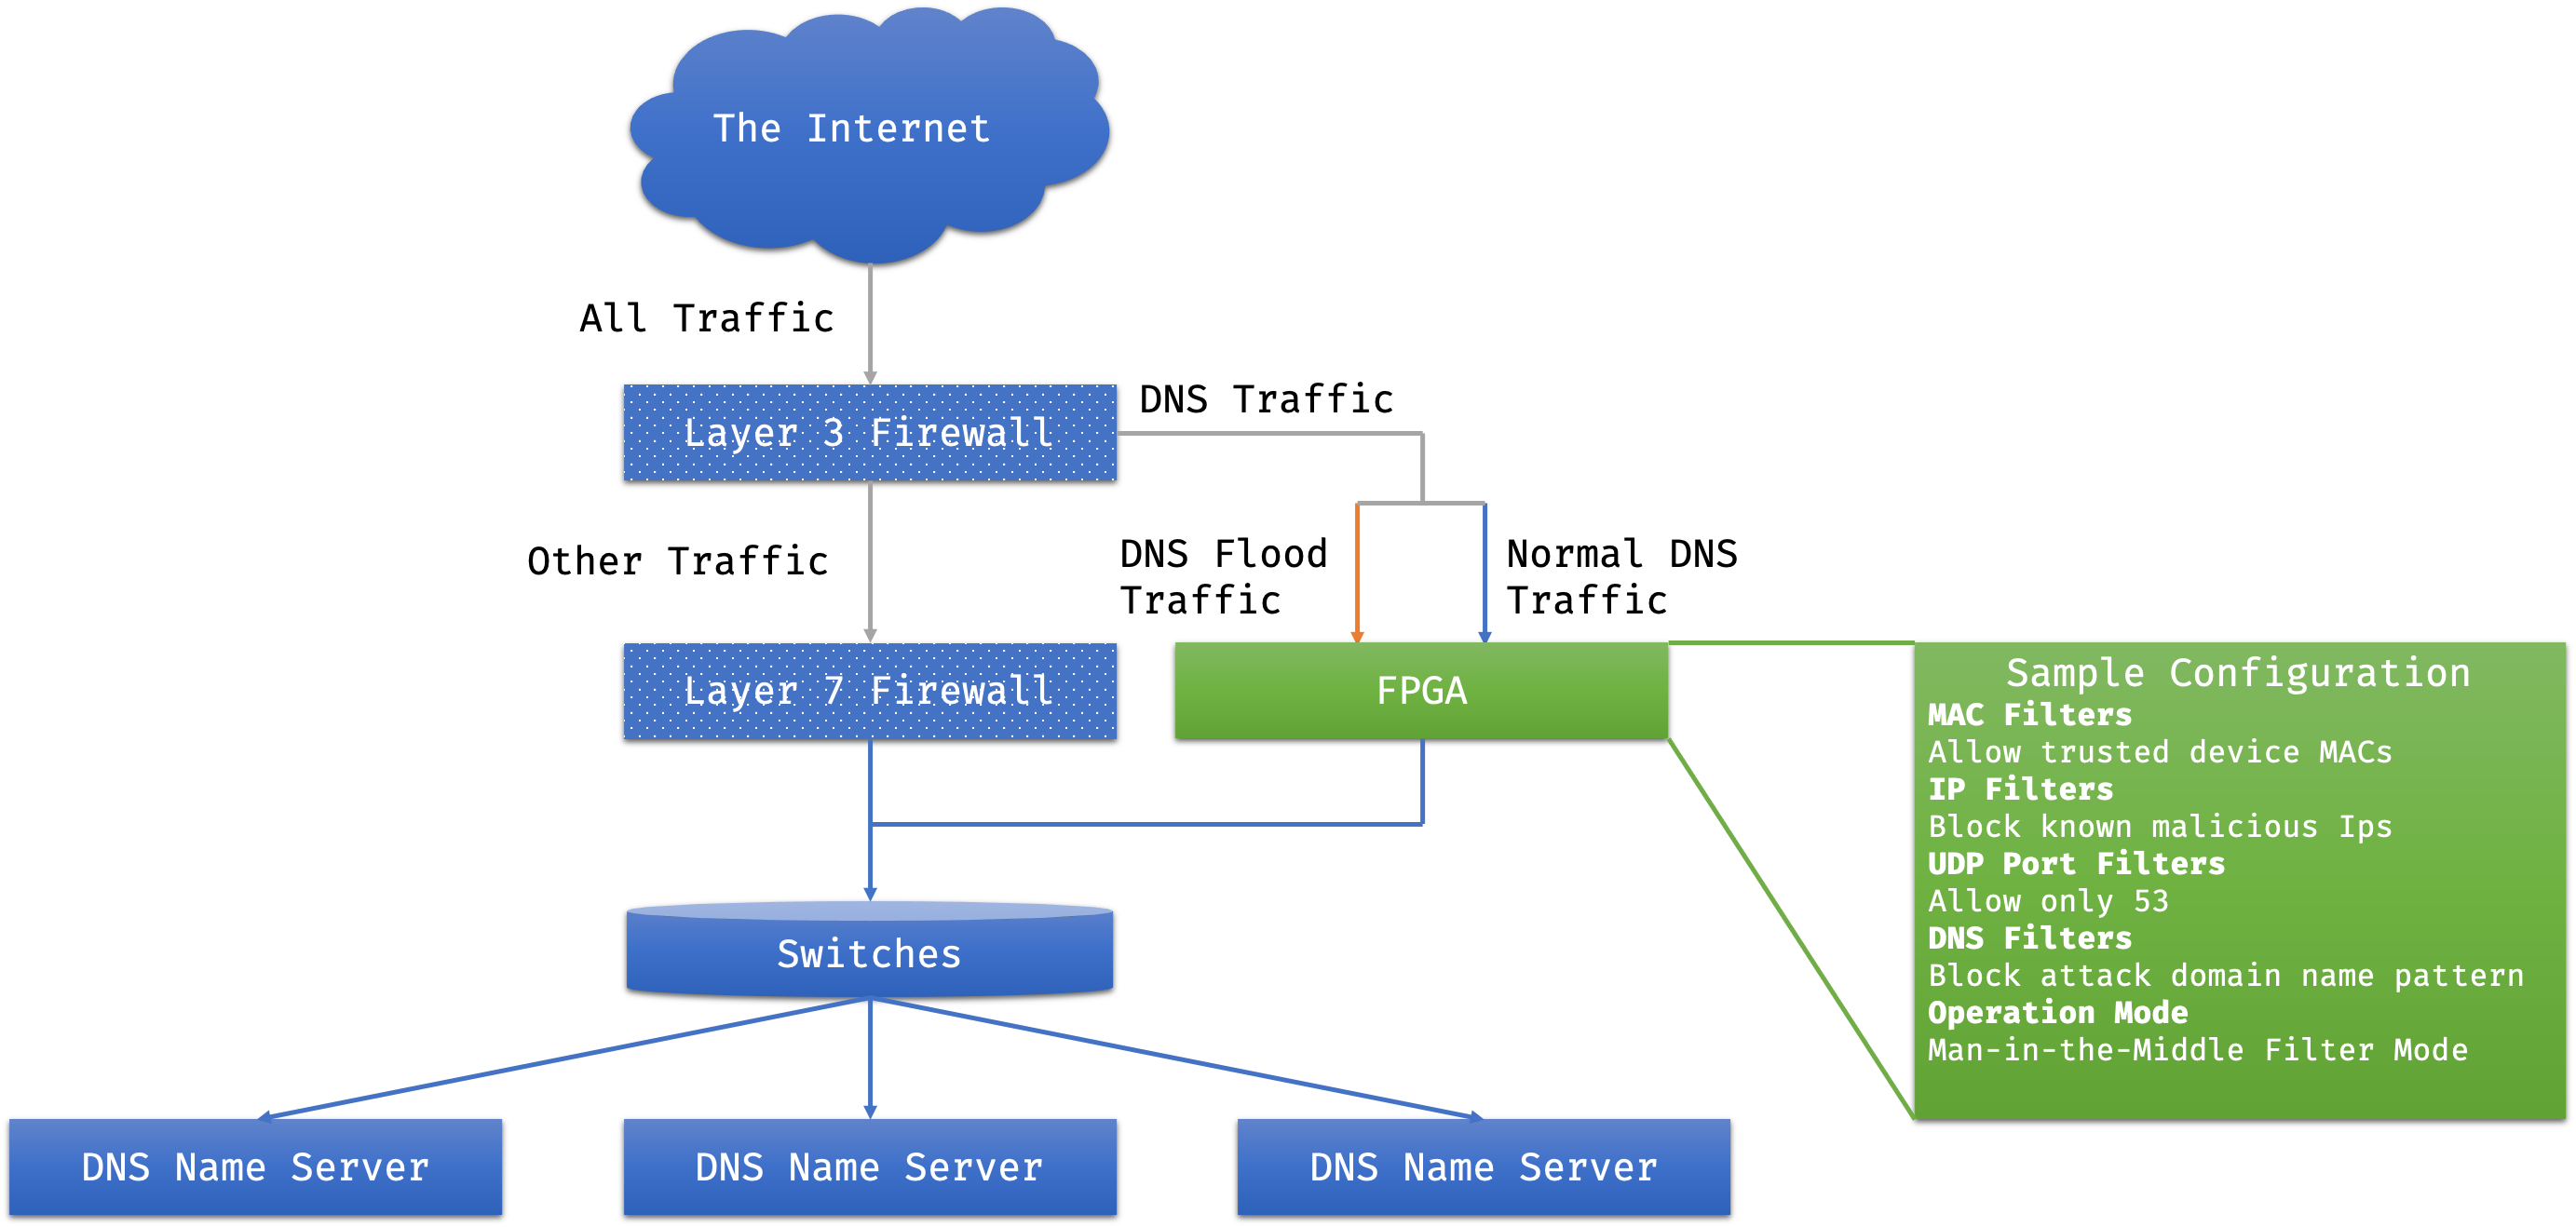
\includegraphics[width=1.1\textwidth]{imgs/man-in-the-middle-amp-topology.png}}
  \caption{Man-in-the-Middle DNS Name Server FPGA sample topology - FPGA on the side}
  \label{fig:dns-flood-man-in-the-middle-asic}
\end{figure}

\chapter{Implementation}

In this chapter, we will be discussing implementation details of the FPGA-based system, including hardware engineering and debugging processes, as well as software development and integration steps.

\section{Hardware Implementation}
\label{section:implementation-hardware-implementation}

\subsection{Finite State Machine (FSM) Implementation}

\begin{figure}[h!]
  \makebox[\textwidth][c]{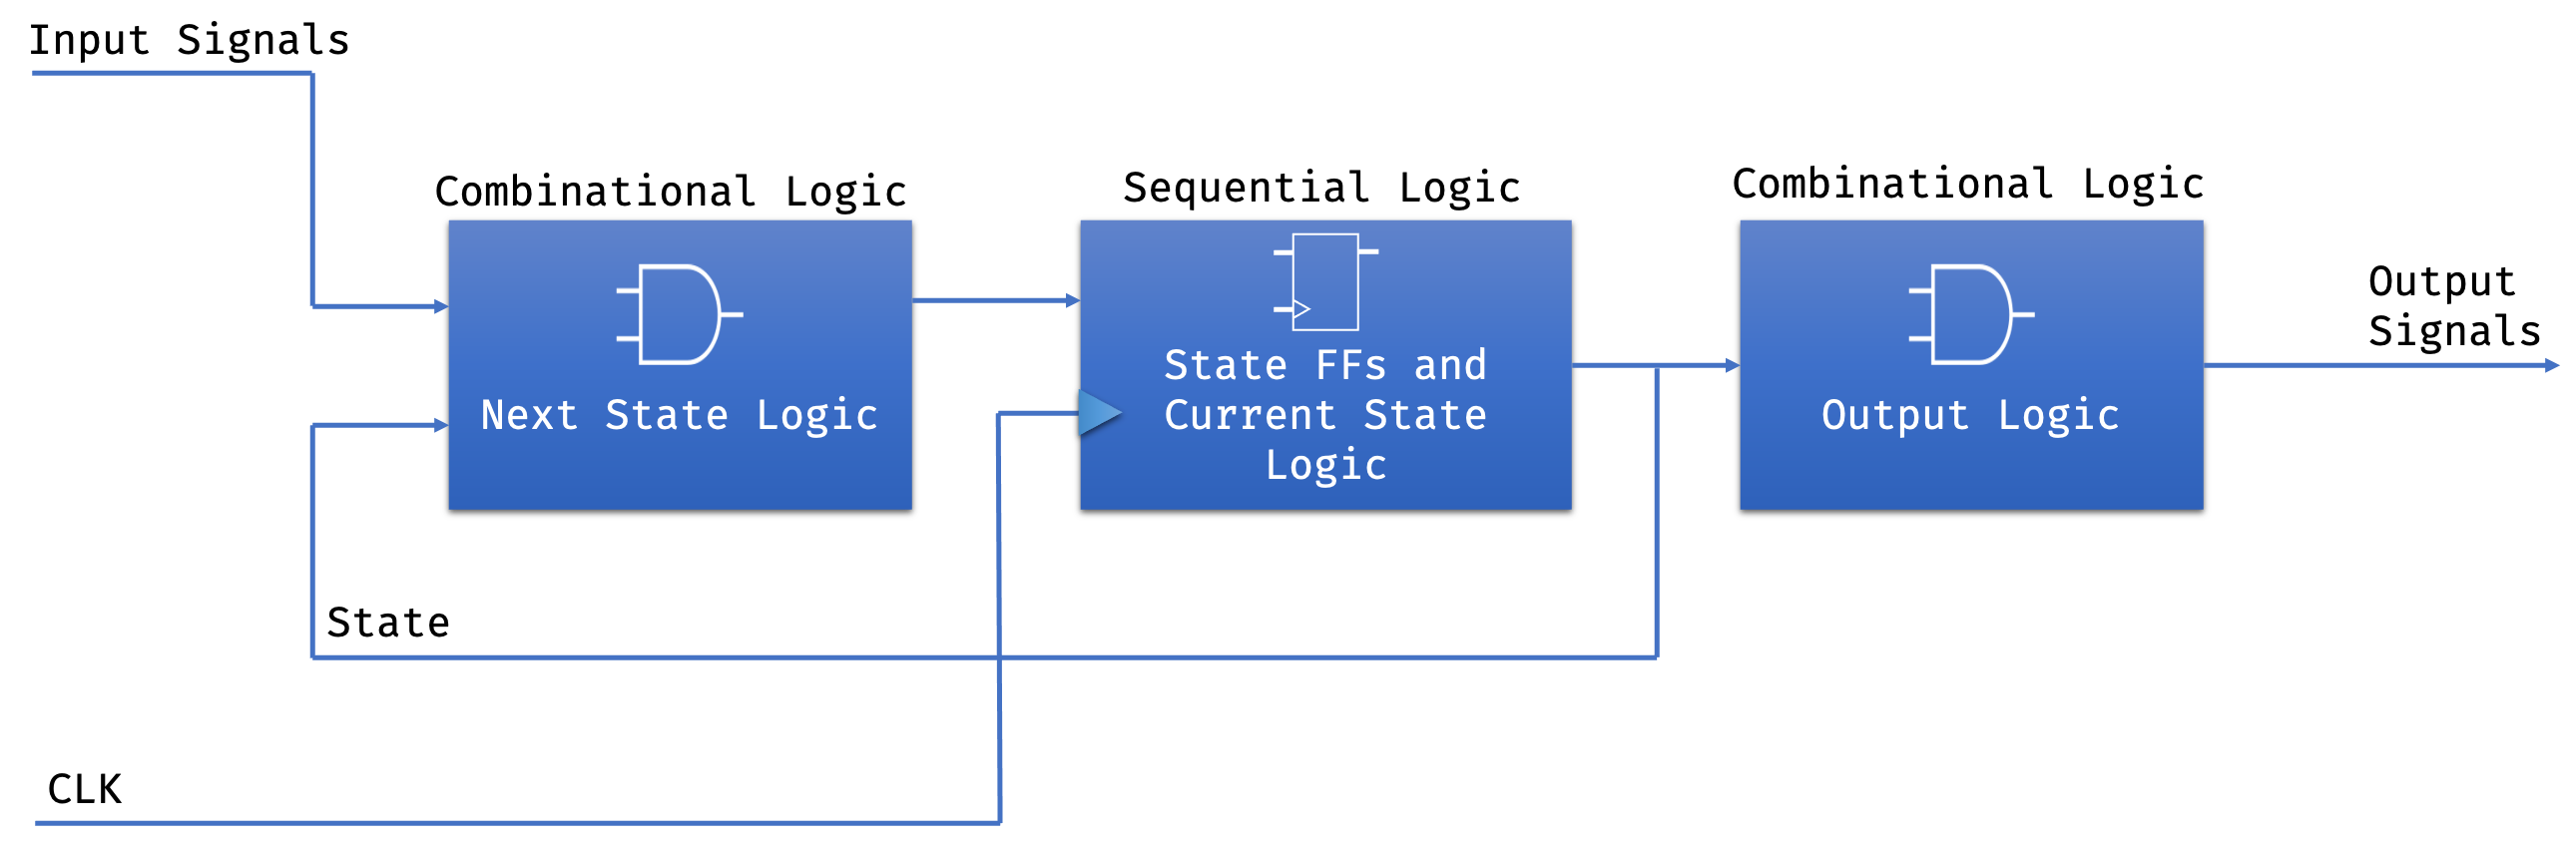
\includegraphics[width=\textwidth]{imgs/FSM-impl.png}}
  \caption{Final State Machine Hardware Implementation}
  \label{fig:fsm-impl}
\end{figure}

FSM is one of the most commonly used design technique in stateful logic hardware circuits. More specifically, a hardware implementation of a $n$-state FSM requires three main logic blocks, as shown in Figure \ref{fig:fsm-impl}:
\begin{itemize}
    \item Next State Logic : a block of combinational circuit to determine the next state.
    \item State FFs and Current State Logic : a set of registers storing state information and a sequential logic circuit operating input signals based on the state. The number of FFs used is dependent on the encoding method, varying from $\ceil*{\log_2 n}$(binary encoded) - $n$(one-hot encoded).
    \item Output Logic : another stateless combinational circuit to output processed signals.
\end{itemize}

\begin{figure}[h!]
    \centering
    \begin{minipage}{0.32\textwidth}
        \centering
        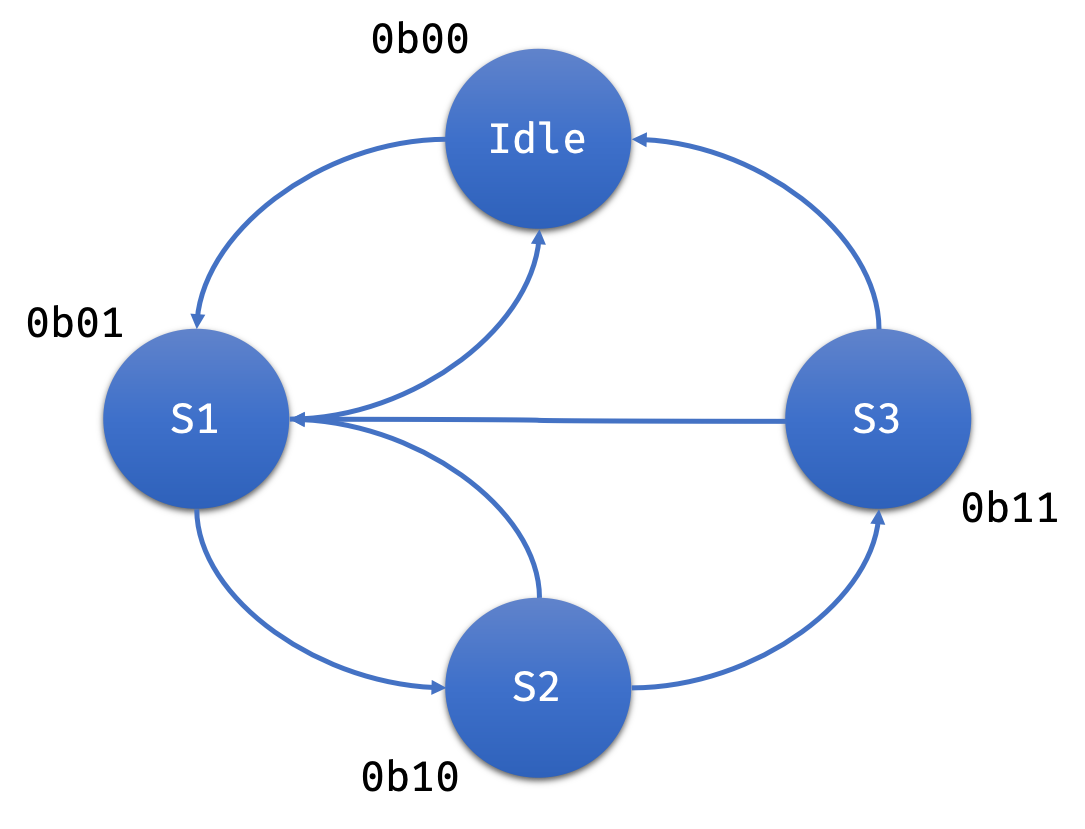
\includegraphics[width=\linewidth]{imgs/binary-encoding-fsm.png}
    \end{minipage}%
    \begin{minipage}{0.32\textwidth}
        \centering
        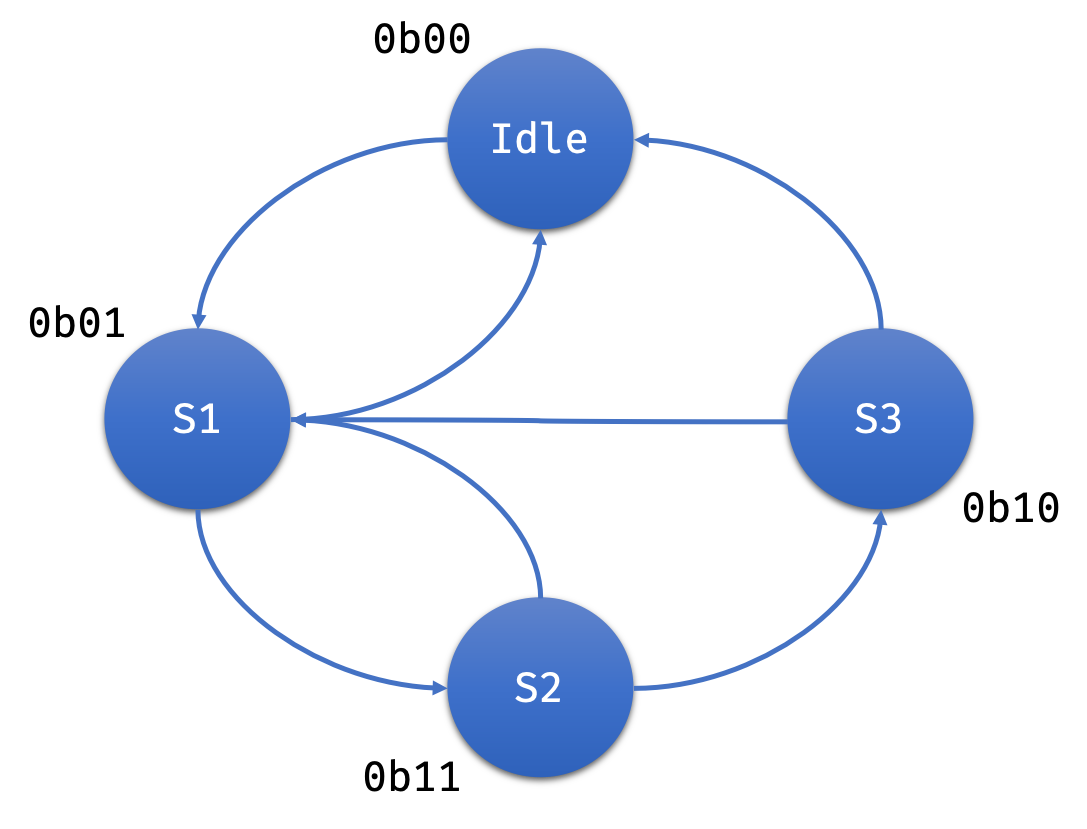
\includegraphics[width=\linewidth]{imgs/grey-encoding-fsm.png}
    \end{minipage}
    \begin{minipage}{0.35\textwidth}
        \centering
        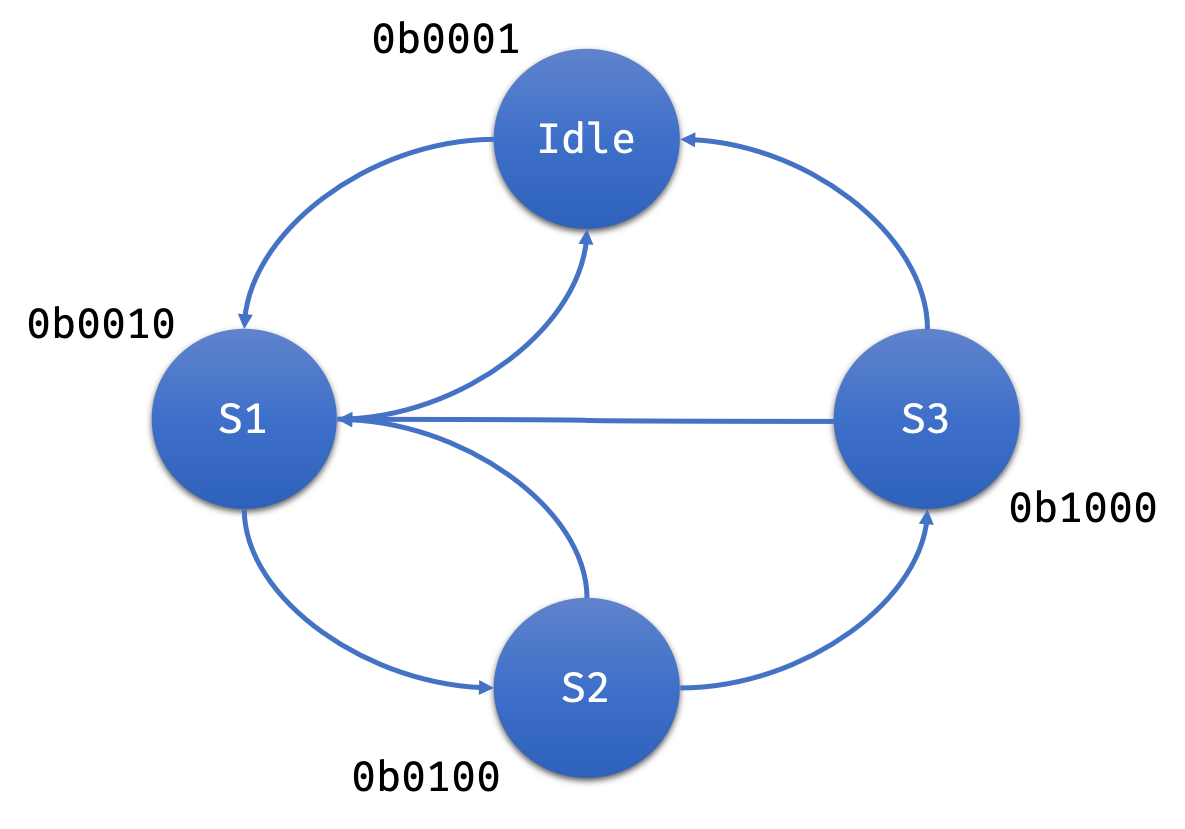
\includegraphics[width=\linewidth]{imgs/one-hot-fsm.png}
    \end{minipage}
    \caption{Binary-Encoded, Grey-Encoded and One-Hot-Encoded FSM}
    \label{fig:binary-grey-one-hot-encoded-FSM}
\end{figure}

With regards to the number of FFs in the state register, there are three main encoding methods shown in Figure \ref{fig:binary-grey-one-hot-encoded-FSM}, namely binary encoding, grey encoding and one-hot encoding.

Binary encoding is the most intuitive one to use when assigning numerical value to sequential states, and we are using as few bits as possible to encode the states. For an $n$-state FSM, binary encoding them sequentially shall yield $\ceil*{\log_2 n}$ bits. With the $4$-state FSM shown on the left side of Figure \ref{fig:binary-grey-one-hot-encoded-FSM}, $\ceil*{\log_2 4} = 2$ FFs would be needed. Binary encoding uses the least amount of memory, but the transitions can be very strict with timing\footnote{See Section \ref{section:implementation-hardware-debugging} for more information on hardware timing constraints \label{foot:timing-constraints}} in cases like going from $\mathtt{0x7f}$ to $\mathtt{0x80}$, with 8 bits to drive within one clock cycle (7 bits to set 0 and 1 bits to set 1).

Grey encoding consists of a sequence where only one bit shall change between the current value and next. This encoding developed aiming to minimise the bit flips when transitioning states so as to further relief the timing constraints and reduce dynamic power consumption\footref{foot:timing-constraints}. Notice the difference of encoding at State $S2$ and $S3$ in between the left FSM and the middle FSM in Figure \ref{fig:binary-grey-one-hot-encoded-FSM}, the grey-encoded FSM encodes $S2$ as $\mathtt{0b11}$ instead of $\mathtt{0b10}$ to ensure $S1 (\mathtt{0b01})\xrightarrow{}S2(\mathtt{0b11})$ flips only one bit, and similarly for $S2 (\mathtt{0b11})\xrightarrow{}S3(\mathtt{0b10})$.

Lastly, one-hot encoding is a scheme where each bit represents one single state. Thus, at any point in time, there shall only be one VCC (1) in states, while all other bits shall be Ground (GND) (0). With reference to the $4$-state FSM on the right side of Figure \ref{fig:binary-grey-one-hot-encoded-FSM}, the four states are encoded as $\mathtt{0b0001}$, $\mathtt{0b0010}$,  $\mathtt{0b0100}$ and $\mathtt{0b1000}$. This encoding method seems inefficient as encoding a $n$-state FSM requires $n$ FFs. However, one-hot encoding particularly useful in strict timing scenarios and simpflies the stimulus logic\footref{foot:timing-constraints}. The bits represents the states directly, and there shall be no state-decoding delay.

\begin{lstlisting}[language=VHDL, caption=One-Hot Encoded FSM Minimal Example in \proglang{VHDL}, label={lst:one-hot-fsm-minimal}]
TYPE state_t IS (IDLE, START, RUN, DONE);

ATTRIBUTE enum_encoding : STRING;
ATTRIBUTE enum_encoding OF state_t : TYPE IS "one-hot";

SIGNAL s, sin : state_t;

stim : PROCESS (clk)
BEGIN
  IF rising_edge(clk) THEN
    CASE s IS
      WHEN IDLE =>
        sin <= START;
      WHEN START =>
        sin <= RUN;
      WHEN RUN =>
        sin <= DONE;
      WHEN DONE =>
        sin <= IDLE;
    END CASE;
  END IF;
END PROCESS;

reg : PROCESS (clk)
BEGIN
  IF falling_edge(clk) THEN
    s <= sin;
  END IF;
END PROCESS;
\end{lstlisting}

Typically, we can provide behavioural description of the FSM states in \proglang{VHDL} and the synthesizer would be able to decide the encoding based on the complexity of the algorithm and the number of states. However, in certain cases where timing constraints are strict, we will have to specify encoding methods precisely via providing a signal description of the state registers.

Listing \ref{lst:one-hot-fsm-minimal} is a minimal example of One-Hot Encoded FSM in \proglang{VHDL}. Note that at line $4$ we set the attribute specifically to \code{one-hot}, and the synthesizer would generate One-Hot-Encoded FSM netlist accordingly. It is also worth noting that we store state \code{s} changes in signal \code{sin} on a rising clock edge and refresh the current state \code{s} on a falling edge. This is an attempt to make sure signal \code{s} would not run into metastability in a clock cycle when it is instantly used after modification\footnote{See Section 4.2 for more information on signal metastability in hardware}.

FSM is implemented in most components within the FPGA-based system, as parsing, processing and constructing network packets are all sequential logic and fits nicely with the stateful design of FSM.

\subsection{Top Level Module and Clock Divider}

Figure \ref{fig:top-level-design} shows the implemented top-level design of the FPGA. As a streamlined packet processing system, the components are connected linearly as the packet flows from the incoming PHY receiver to the outgoing PHY transmitter.

\begin{landscape}
\begin{figure}[h!]
  \centering
  \includegraphics*[viewport={0 0 950 600}, height=\textwidth, width=2\textheight, keepaspectratio]{imgs/top-level-module.png}
  \caption{Top Level Module Overview - 1}
  \label{fig:top-level-design}
\end{figure}
\begin{figure}[h!]
  \ContinuedFloat
  \centering
  \includegraphics*[viewport={950 0 1900 600}, height=\textwidth, width=2\textheight, keepaspectratio]{imgs/top-level-module.png}
  \caption{Top Level Module Overview - 2}
  \label{fig:top-level-design}
\end{figure}
\begin{figure}[h!]
  \ContinuedFloat
  \centering
  \includegraphics*[viewport={1900 0 2850 600}, height=\textwidth, width=2\textheight, keepaspectratio]{imgs/top-level-module.png}
  \caption{Top Level Module Overview - 3}
  \label{fig:top-level-design}
\end{figure}
\end{landscape}

\begin{lstlisting}[language=VHDL, caption=Snippet of Clock Divider \code{clock.vhd}, label={lst:clock-vhd}]
ARCHITECTURE rtl OF clock IS
  SIGNAL clk_divider : unsigned(1 DOWNTO 0) := (OTHERS => '0');
BEGIN

  div : PROCESS (i_clk)
  BEGIN
    IF (rising_edge(i_clk)) THEN
      clk_divider <= clk_divider + 1;
    END IF;
  END PROCESS div;

  o25_clk <= clk_divider(1);
  o50_clk <= clk_divider(0);
 
END rtl;
\end{lstlisting}

As seen at the bottom of left of Figure \ref{fig:top-level-design}, \code{inst\_clock} is the clock divider component of the system. With reference to the Digilent Arty A7-35T manual\cite{digilent-arty}, a single crystal oscillator of $100$ MHz is connected to the board via pin E3. Considering system stability and overall design difficulties, we set the Artix-7 FPGA core to the default $50$ MHz Speedgrade 1 as per Xilinx clocking documentation \cite{xilinx-7-clocking}. Moreover, the interfacing PHY chip, Texas Instruments (TI) DP83848J, operates under a $25$ MHz clock when using MII ($50$ MHz when using Reduce MII (RMII)), which needs to be generated by the circuit and send to pin X1\cite{texas-instruments-dp83848x}. Therefore, we would need to introduce a oscillator signal processor to generate the clock we want in different domains of the system. As laid out in Listing \ref{lst:clock-vhd}, The clock divider operates upon the rising edge of the oscillator and produces slower clock using an internal unsigned rollover counter. Note that the clock divider is implemented as simple as possible without overflow checks to minimise the processing skew added to the FPGA fast clock path.

\subsection{PHY MII-family Interface, Receiver and Sender Peripheral}

As described earlier, Arty-A7 35T has an on-chip Ethernet PHY ASIC peripheral (TI DP83848J), which operates under two interfaces, two Cat 5 speed grades and two duplex modes: RMII / MII, $10$ / $100$ Mbps and half/full duplex respectively \cite{texas-instruments-dp83848x}. All three settings can be configured via functional pins \code{LED\_LINK}, \code{LED\_SPEED} and \code{MII\_MODE}. In this project, we configure the PHY chip to operate with MII interface, $100$ Mbps full-duplex PHY link.

The MII-family interface is standard by IEEE 802.3u \cite{ieee802.3ethernet-2018} as the interface to connect a Ethernet Media Access Control (MAC) block to a PHY ASIC. It is considered to be an universal abstraction interface above various physical network medias (i.e. twisted pair, fiber optic and etc.). With the MII-family interface, any MAC hardware/software can connect to any PHY independent of the network signal transmission media.

The main receiving and transmitting signals on the interface includes:
\begin{itemize}
    \item \code{CRS}: Carrier Sense
    \item \code{COL}: Collision, which would not be used in full-duplex connections
    \item \code{RX\_CLK}, \code{TX\_CLK}: Receive / Transmit Clock
    \item \code{RXD[0-3]}: Receive Data [0-3],  (4 bits per clock cycle)
    \item \code{TXD[0-3]}: Transmit Data [0-3],  (4 bits per clock cycle)
    \item \code{RX\_DV}: Receive Data Valid (GND on this signal means data received on \code{RXD[0-3]} are just noise on the PHY)
    \item \code{TX\_EN}: Transmit enable (VCC on this signal means data provided on \code{TXD[0-3]} will be sent to the wire)
    \item \code{RX\_ER}, \code{TX\_ER}: Receive / Transmit Error (VCC on this signal means the PHY has received undecodable data / was unable to transmit data, possibly due to broken connections or unsuccessful negotiations)
\end{itemize}

\begin{figure}[h!]
  \makebox[\textwidth][c]{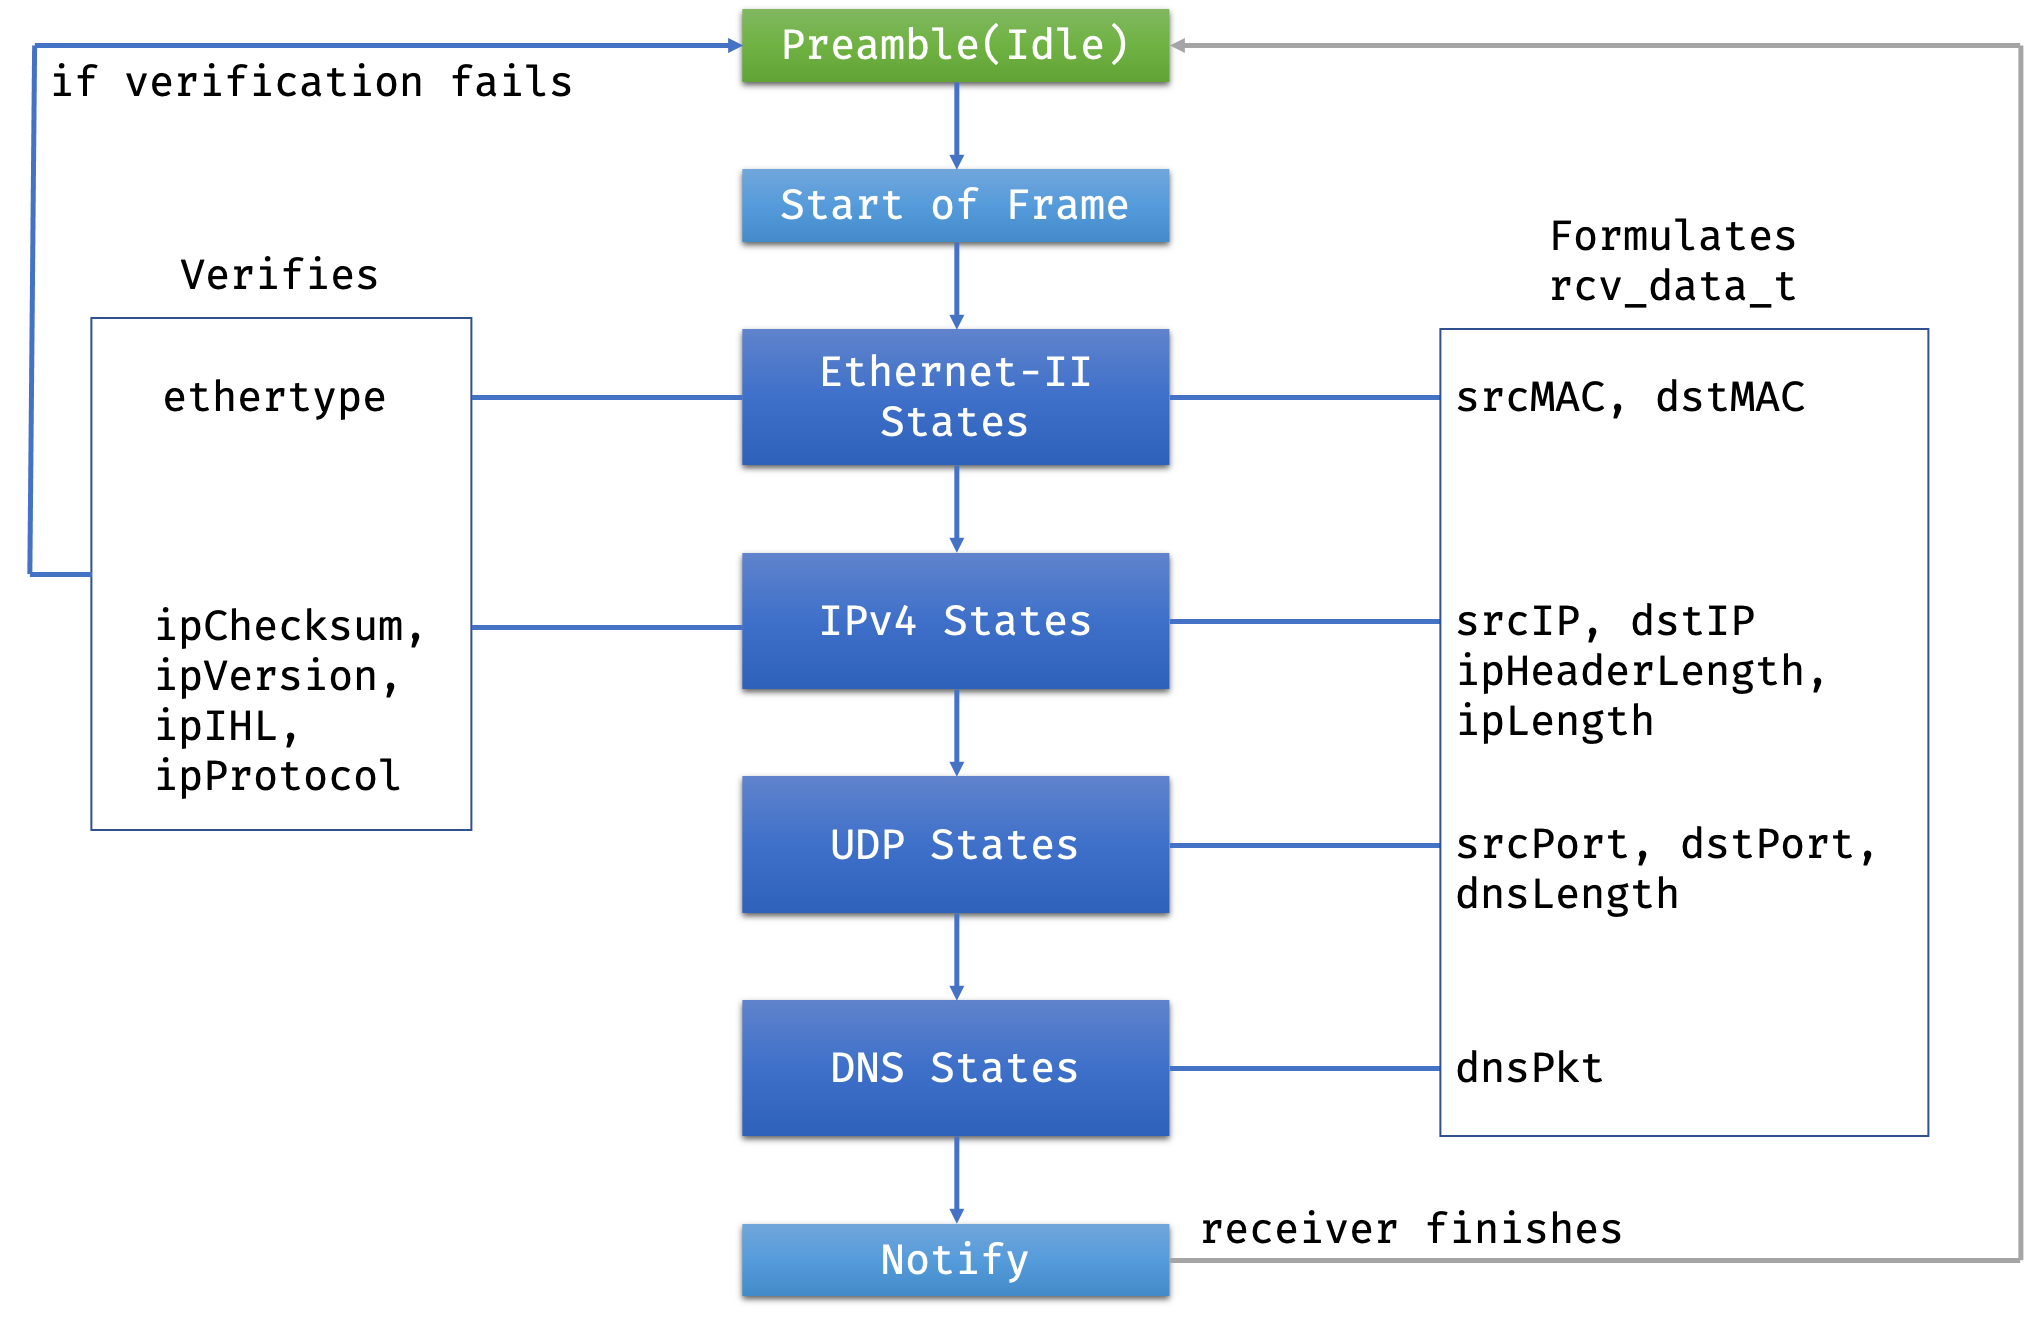
\includegraphics[width=0.8\textwidth]{imgs/rcv-fsm.png}}
  \caption{\code{mac\_rcv.vhd} Module FSM Overview}
  \label{fig:rcv-fsm}
\end{figure}

Using the FSM sequential logic, we implemented our Receiver FSM as shown in Figure \ref{fig:rcv-fsm}. When \code{RX\_DV} is at VCC level, the receiver will start listening for Ethernet-II preambles at state \code{Preamble} and proceed with state transitions accordingly. During the parsing states, the receiver will analyse the packet as nibbles (4 bits) comes in from \code{RXD}, forms a \code{rcv\_data\_t} and checks for packet correctness at numerous checkpoints, including \code{ethertype}, \code{ipChecksum} and etc. As mentioned previously in design Section \ref{section:design-system-design-hardware}, the \code{dnsPkt} struct is limited to $1024$ bits (128 bytes) for the ease of signal transfer across components under strict timing requirements at the \code{Notify} state. Once the all verification passes and the sturct \code{rcv\_data\_t} is properly constructed, the component would notify its predecessor by setting \code{EL\_DV} to high and return to the state \code{Preamble(Idle)}, ready for the next packet.

\begin{figure}[h!]
  \makebox[\textwidth][c]{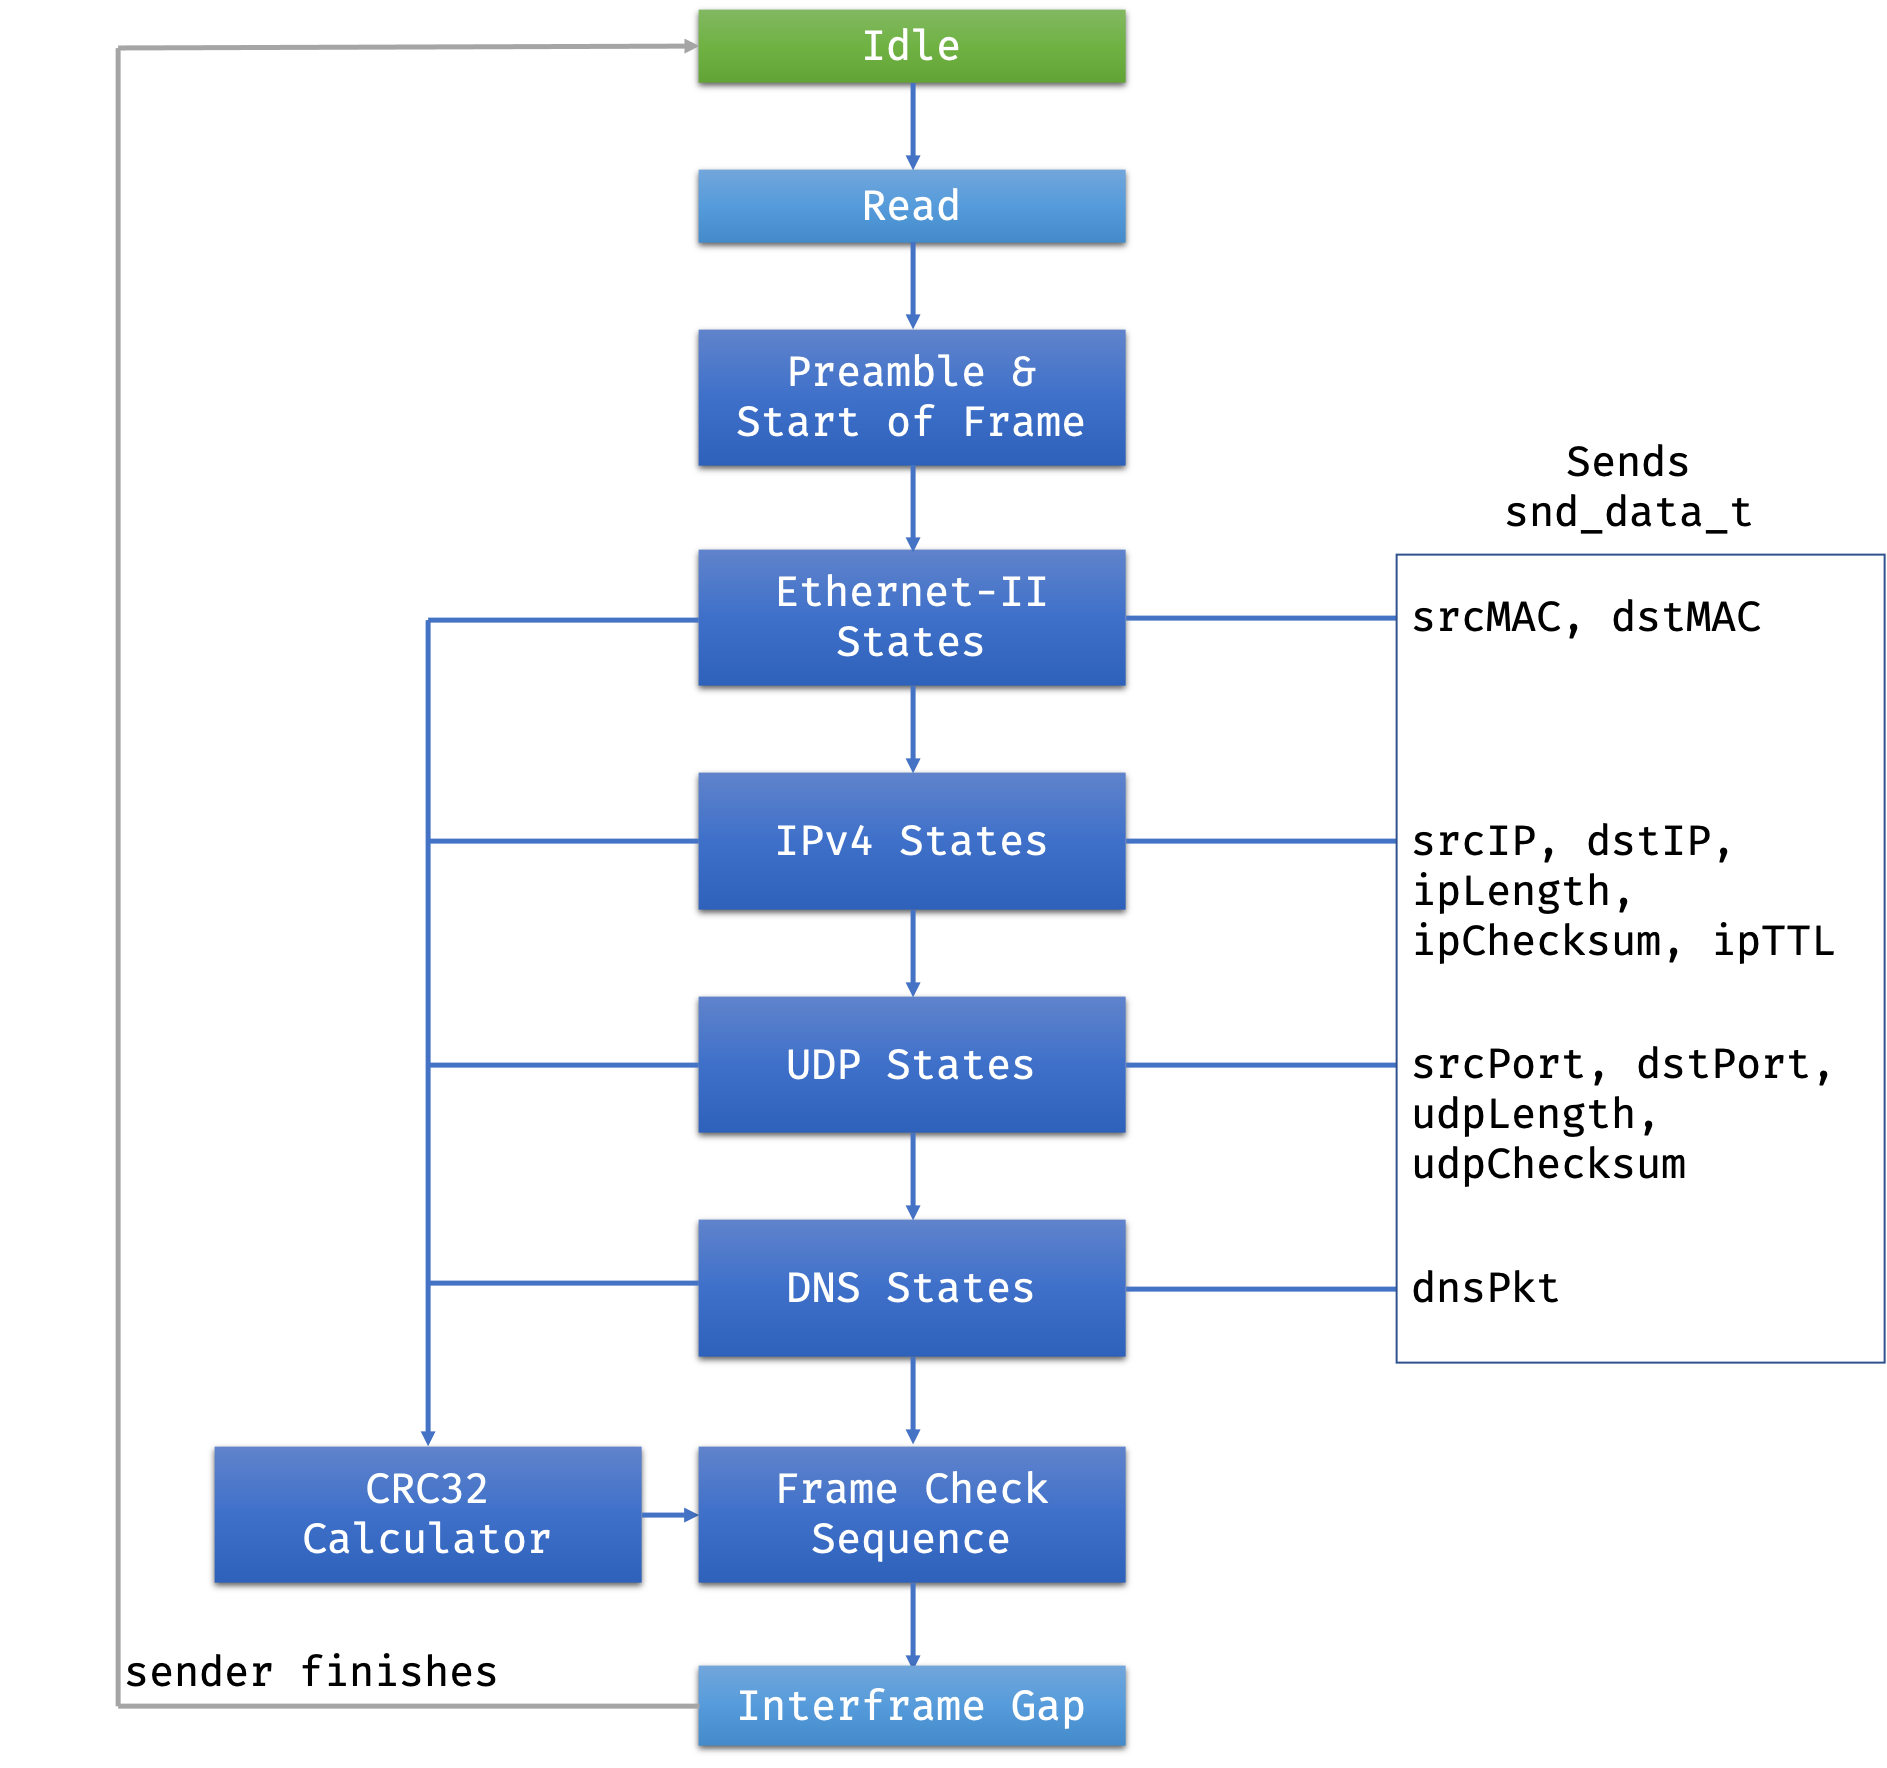
\includegraphics[width=0.8\textwidth]{imgs/snd-fsm.png}}
  \caption{\code{mac\_snd.vhd} Module FSM Overview}
  \label{fig:rcv-fsm}
\end{figure}

Similarly, we also implemented the Sender interfacing with the PHY transmitter with a FSM shown in Figure \ref{fig:rcv-fsm}. While the internal logic is in reverse order, sending signals to the interfaces rather than receiving, the general states of the FSM are alike. Note that the Sender operates based on a sending struct named \code{snd\_data\_t} with checksums and TTLs calculated and metadata imported from previous steps at state \code{Read}. As the sender pulls up \code{TX\_EN} and sends nibble streams to the \code{TXD} interface, the CRC32 calculator would also receive the stream and calculates the next-state FSM within the clock cycle. When all DNS payload has been transmitted, the 32-bit (8 byte) CRC sequence will be emitted by the calculator component and appended to the packet. Lastly but easily forgotten, Ethernet-II requires a interframe gap of 12 octets (24 nibbles) of \code{TX\_EN} at GND before a new packet can be transmitted. Not following the procedure properly would cause the next packet to be discarded by the intended recipients.

\subsection{Clock-Domain-Crossing FIFO}

One of the most common methods of transferring data across clock domains is to use a FIFO buffer. In hardware implementation, a CDC FIFO is usually a dual port RAM that operates separately with a read CLK and a write CLK. In our minimalistic CDC FIFO design shown in Listing \ref{lst:fifo-rcv-vhd}, we introduce two pairs of behavioural circuit corresponding to reading and writing to the FIFO. Each pair consists of a Next-State-Logic (NSL) which detects and operate read and write on the FIFO, and a register (REG) process that updates the index pointer state of the FIFO. Whenever there is packet left to be processed in the FIFO, the \code{buf\_not\_empty} signal would be pulled to VCC in order to let the predecessor aware of the new task at hand.

\begin{lstlisting}[language=VHDL, caption=Snippet of FIFO \code{FIFO\_receive.vhd}, label={lst:fifo-rcv-vhd}]
  fifo_wnsl : PROCESS (wclk)
  BEGIN
    IF (rising_edge(wclk)) THEN IF (w_en = '1') THEN
      ... ELSE ...
    END IF; END IF;
  END PROCESS;

  fifo_wreg : PROCESS (wclk)
  BEGIN
    IF falling_edge(wclk) THEN
      w_index <= win_index;
    END IF;
  END PROCESS;

  fifo_rnsl : PROCESS (rclk)
  BEGIN
    IF (rising_edge(rclk)) THEN IF (r_en = '1') THEN
        ... ELSE ...
    END IF; END IF;
  END PROCESS;

  fifo_rreg : PROCESS (rclk)
  BEGIN
    IF falling_edge(rclk) THEN
      r_index <= rin_index;
    END IF;
  END PROCESS;

  buf_not_empty <= '0' WHEN w_index = r_index ELSE '1';
\end{lstlisting}

In particular, we omit the commonly used Almost Full (AF) and Almost Empty (AE) flags in our FIFO as a implementation decision to discard the all 8 packets left unprocessed within the FIFO when index pointers collide, meaning the FIFO is full and unable to receive new packets. This is unlikely to happen as the core operates at much higher speed with 2 times lower processing time than the PHY clock domain. Hence, it is almost impossible to flood the core with too many packets to process. On the rare occasion it does happen, there would be no difference to discard new incoming packets or current packets in the FIFO as they are of equal importance. This also omits extra logic to check and monitor the FIFO status, which could yield minor latency improvements to the design.

\subsection{Core Input Processor}

\begin{figure}[h!]
  \makebox[\textwidth][c]{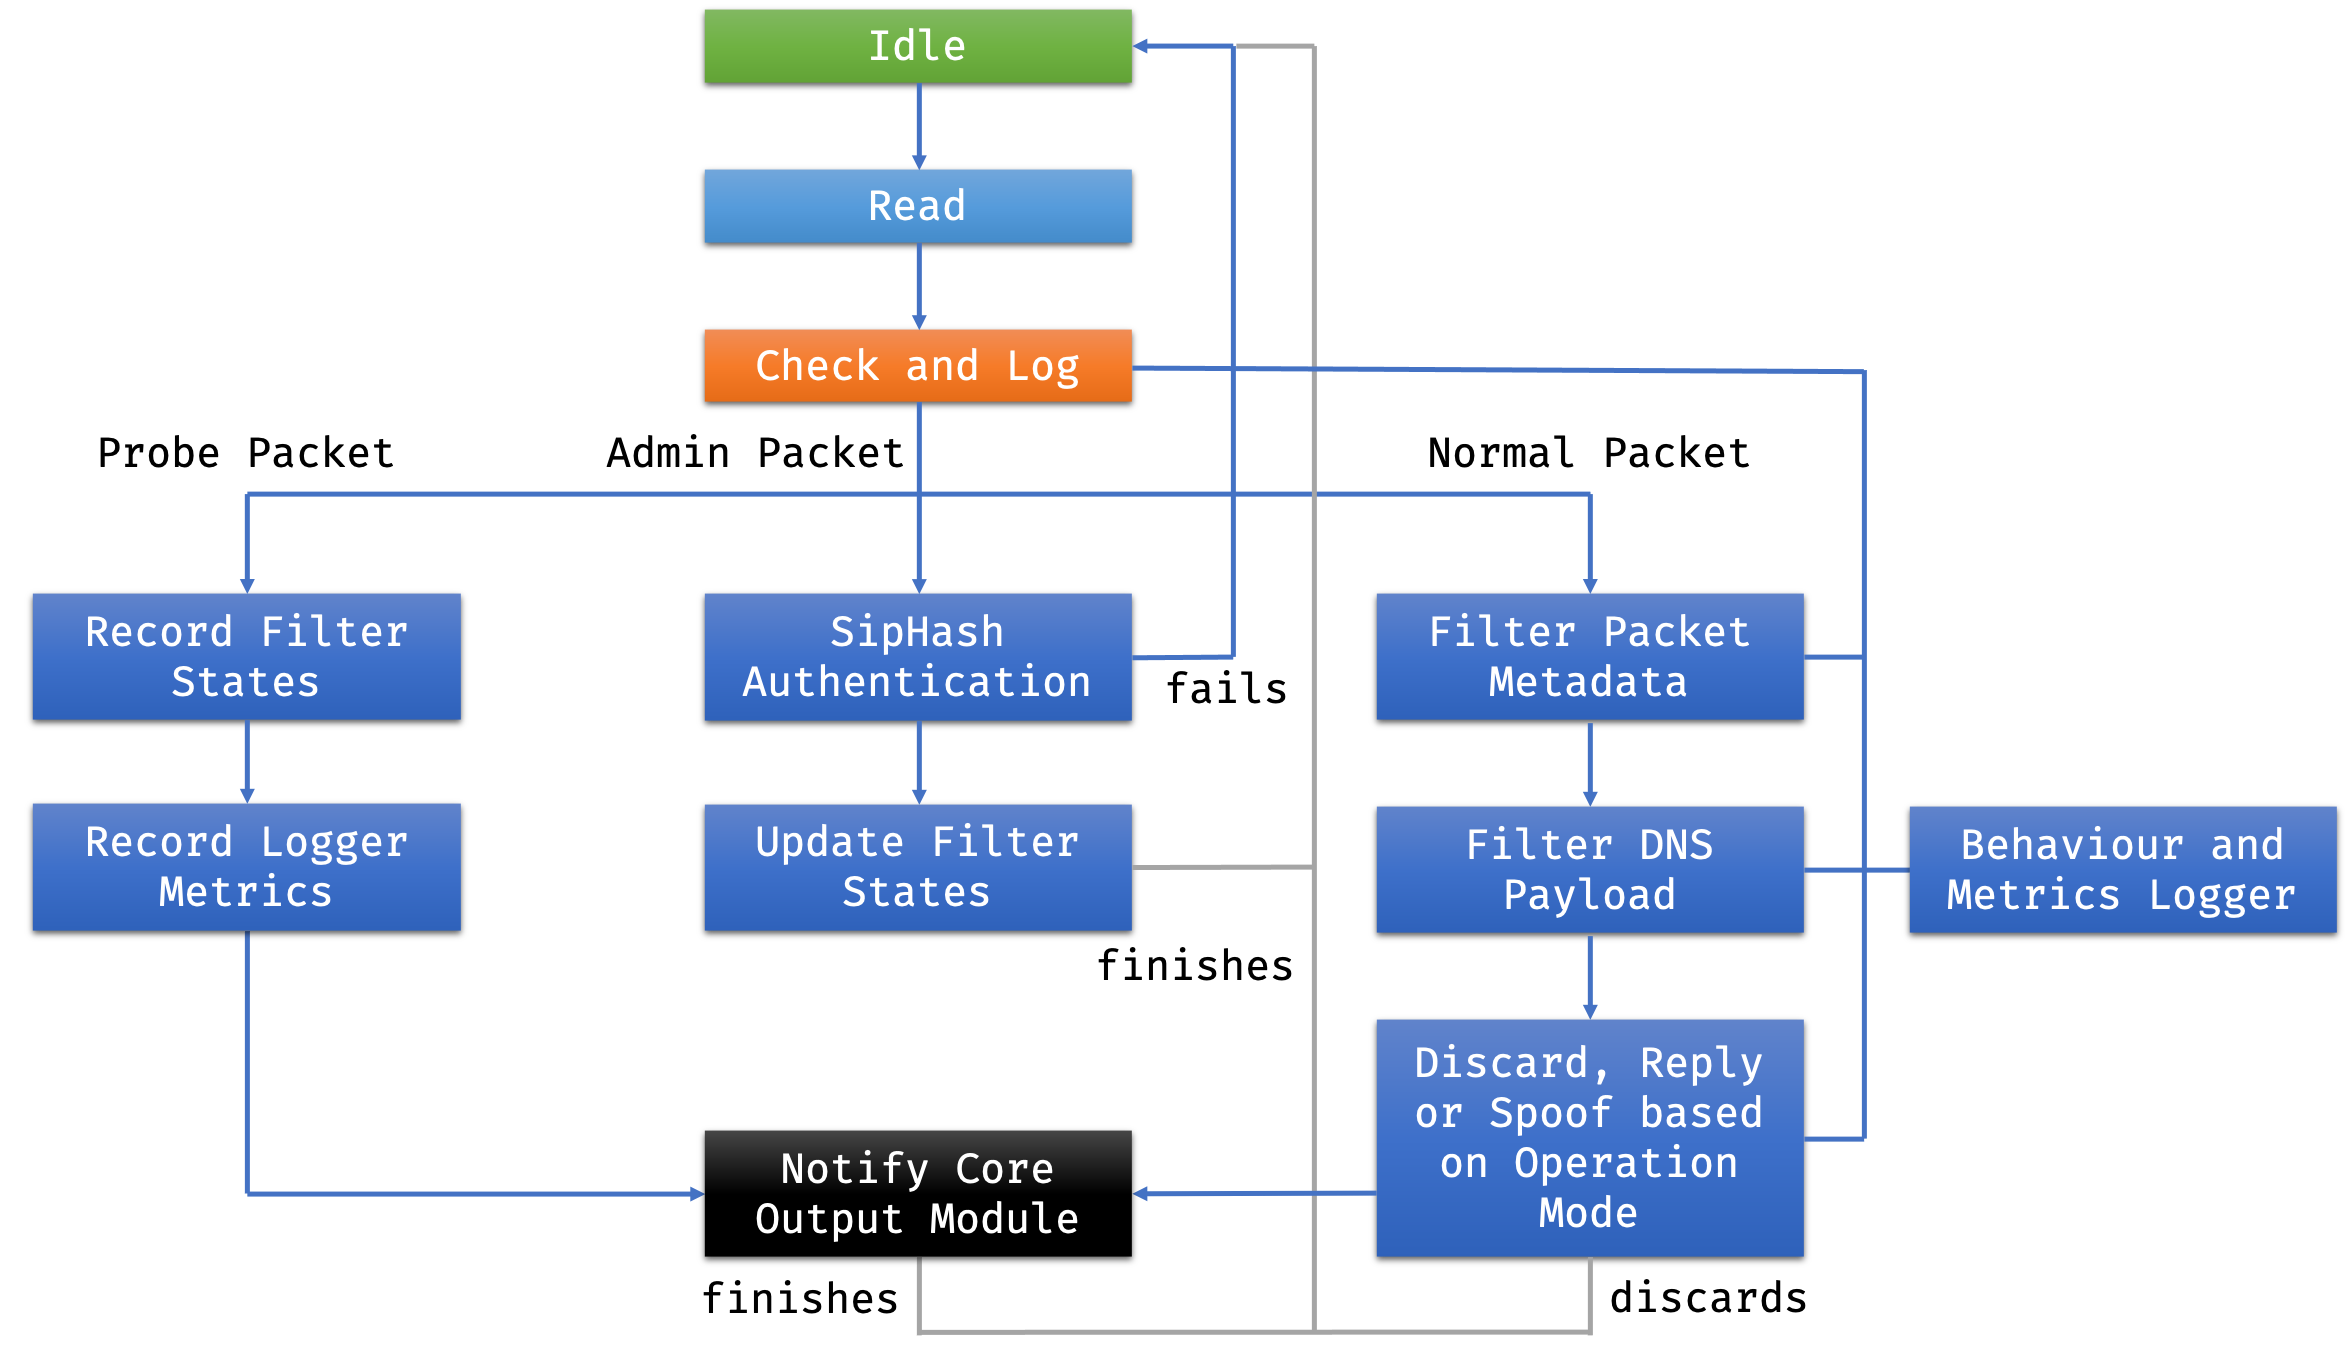
\includegraphics[width=\textwidth]{imgs/corein-fsm.png}}
  \caption{\code{i.vhd} Module FSM Overview}
  \label{fig:corein-fsm}
\end{figure}

The Core Input Processor is where the core processing and handling of network packets happens. Its high-level FSM is demonstrated in Figure \ref{fig:corein-fsm}. As the FIFO signals the \code{corein} unit, the full packet struct of \code{rcv\_data\_t} will be fetched at the \code{Read} state. The processor will then log the packet and identify the packet into three main categories:
\begin{itemize}
    \item Probe Packet : Packet that probes the FPGA for its current configuration and up-to-date metrics.
    \item Admin Packet : Packet sent from the FPGA administrators that carries new information for filters and operation mode configurations.
    \item Normal Network Packet : Packet that shall be checked and acted upon based on current on-board filter and operation configurations.
\end{itemize}

For a normal network packet received, it will be filtered / checked in the areas of MAC addresses, IP addresses, UDP ports, DNS headers and domain names. The filter will compare these information to given lists in the configuration. Dependent on the lists being blacklists or whitelists, the processor will provide a binary decision at the end of each procedure. By the end of all checks, the checkers will reach a final binary decision of pass or not pass. Then, based on the FPGA operation mode (man-in-the-middle filter mode, man-on-the-side spoof mode), the FPGA will take one of the four actions as instructed: forward the payload, forward the DNS transaction, spoof a DNS transaction, or discard the packet. Depending on the result, the core output module will be notified accordingly to deal with packet checksums and other relevant metadata. This is estimated to take at least 10 clock cycles (200 nanoseconds) under the best cases, and at most 120 clock cycles (2400 nanoseconds) with the largest payload and the most complex filters.  

Once a probe packet is logged, the FPGA will pack the current filter configurations and logger metrics by bits in a compact packet and pass on to the core output constructor for checksum calculations in less than 20 clock cycles (400 nanoseconds), relatively quick and straightforward.


\newpage

Admin packet and reference to next subsection

\subsection{SipHash Authentication Component}
\label{section:implementation-hardware-implementation-siphash}


\subsection{Core Output Packet Constructor}
Core Output - Packet Constructor, Checksum generator, size checker, DNS header generation


\section{Hardware Debugging}
\label{section:implementation-hardware-debugging}

Although HDL has many similarities with software programming languages like C and Ada, they are fundamentally different as HDL describes electric circuits which is executed in parallel, while programming languages expresses a sequential set of instructions.

Sequential execution

Clock domain crossing

Timing Constraint

Signal Meta-stability

Variable length comparison in HDL

AND SOMETHING WORKS in SIMULATOR doesn't mena it works?
behavioural simulation and synthesised netlist simulation

Chipscope and LED

.. better read the process.txt

\section{Software Control System}

CLI parser / command execution structure, function pointers

bit manipulation in C/C++, endianess

Other tools developed to streamline software development process

\chapter{Validation and Evaluation}

Power consumption low, performance high

\section{Simulation Unit Test-bench}

\section{Hardware Integration Testing via Software}

\section{Performance Evaluation}

\chapter{Conclusions and Future Work}

\section{Conclusions}

\section{Future Work}
How the project might be continued, but do not give the impression you ran out of time!

\addcontentsline{toc}{chapter}{References}
\printbibliography[title=References]

\appendix

\chapter{Project Demo}

\chapter{Code Listing}

URL \url{https://github.com/magetron/cpu-fpga-nwofle}

\chapter{Original Project Proposal}

\end{document}